\documentclass[a4paper, twoside=true, 12pt]{extreport}
% basics
\usepackage[utf8]{inputenc}
\usepackage[T1]{fontenc}
\usepackage{textcomp}
% \usepackage[dutch]{babel}
\usepackage{url}
\usepackage{hyperref}
\hypersetup{colorlinks=true, pdfstartview=FitV, linkcolor=blue, 
citecolor=black, plainpages=false, urlcolor=black}
\usepackage{graphicx}
\usepackage{float}
\usepackage{booktabs}
\usepackage{enumitem}
\usepackage{parskip}
\usepackage{emptypage}
\usepackage{subcaption}
\usepackage{multicol}
\usepackage{cprotect}
\usepackage{multirow}
\usepackage{verbatimbox}
\usepackage{listings}
\usepackage{xparse}
\usepackage{multirow}
\usepackage[usenames,dvipsnames]{xcolor}

% \usepackage{cmbright}
\usepackage{geometry}
\geometry{a4paper, twoside=true}
\geometry{
 a4paper,
 total={170mm,257mm},
 left=25mm,
 top=20mm, 
 right = 25mm
 }


\usepackage{amsmath, amsfonts, mathtools, amsthm, amssymb}
\usepackage{mathrsfs}
\usepackage{cancel}
\usepackage{bm}
\newcommand\N{\ensuremath{\mathbb{N}}}
\newcommand\R{\ensuremath{\mathbb{R}}}
\newcommand\Z{\ensuremath{\mathbb{Z}}}
\renewcommand\O{\ensuremath{\emptyset}}
\newcommand\Q{\ensuremath{\mathbb{Q}}}
\newcommand\C{\ensuremath{\mathbb{C}}}
\DeclareMathOperator{\sgn}{sgn}
\usepackage{systeme}
\let\svlim\lim\def\lim{\svlim\limits}
\let\implies\Rightarrow
\let\impliedby\Leftarrow
\let\iff\Leftrightarrow
\let\epsilon\varepsilon
\usepackage{stmaryrd} % for \lightning
\newcommand\contra{\scalebox{1.1}{$\lightning$}}
% \let\phi\varphi

\usepackage{titlesec}

\titleformat{\chapter}[hang] 
{\normalfont \fontsize{20pt}{40pt}\bfseries}{\thechapter.}{0.55em}{}   
\titlespacing{\chapter}{0pt}{-30pt}{3px}

\titleformat{\section}[hang]
{\normalfont \fontsize{18px}{18px}\bfseries}{\thesection}{1em}{}
\titlespacing{\section}{0px}{20px}{15px}





% correct
\definecolor{correct}{HTML}{009900}
\newcommand\correct[2]{\ensuremath{\:}{\color{red}{#1}}\ensuremath{\to }{\color{correct}{#2}}\ensuremath{\:}}
\newcommand\green[1]{{\color{correct}{#1}}}



% horizontal rule
\newcommand\hr{
    \noindent\rule[0.5ex]{\linewidth}{0.5pt}
}


% hide parts
\newcommand\hide[1]{}



% si unitx
\usepackage{siunitx}
\sisetup{locale = UK}
% \renewcommand\vec[1]{\mathbf{#1}}
\newcommand\mat[1]{\mathbf{#1}}


% tikz
\usepackage{tikz}
\usepackage{tikz-cd}
\usetikzlibrary{intersections, angles, quotes, calc, positioning}
\usetikzlibrary{arrows.meta}
\usepackage{pgfplots}
\pgfplotsset{compat=1.13}


\tikzset{
    force/.style={thick, {Circle[length=2pt]}-stealth, shorten <=-1pt}
}

% theorems
\makeatother
\usepackage{thmtools}
\usepackage[framemethod=TikZ]{mdframed}
\mdfsetup{skipabove=1em,skipbelow=0em}


\theoremstyle{definition}

\declaretheoremstyle[
    headfont=\bfseries\sffamily\color{ForestGreen!70!black}, bodyfont=\normalfont,
    mdframed={
        linewidth=2pt,
        rightline=false, topline=false, bottomline=false,
        linecolor=ForestGreen, backgroundcolor=ForestGreen!5,
    }
]{thmgreenbox}

\declaretheoremstyle[
    headfont=\bfseries\sffamily\color{NavyBlue!70!black}, bodyfont=\normalfont,
    mdframed={
        linewidth=2pt,
        rightline=false, topline=false, bottomline=false,
        linecolor=NavyBlue, backgroundcolor=NavyBlue!5,
    }
]{thmbluebox}

\declaretheoremstyle[
    headfont=\bfseries\sffamily\color{NavyBlue!70!black}, bodyfont=\normalfont,
    mdframed={
        linewidth=2pt,
        rightline=false, topline=false, bottomline=false,
        linecolor=NavyBlue
    }
]{thmblueline}

\declaretheoremstyle[
    headfont=\bfseries\sffamily\color{RawSienna!70!black}, bodyfont=\normalfont,
    mdframed={
        linewidth=2pt,
        rightline=false, topline=false, bottomline=false,
        linecolor=RawSienna, backgroundcolor=RawSienna!5,
    }
]{thmredbox}

\declaretheoremstyle[
    headfont=\bfseries\sffamily\color{RawSienna!70!black}, bodyfont=\normalfont,
    numbered=no,
    mdframed={
        linewidth=2pt,
        rightline=false, topline=false, bottomline=false,
        linecolor=RawSienna, backgroundcolor=RawSienna!1,
    },
    qed=\qedsymbol
]{thmproofbox}

\declaretheoremstyle[
    headfont=\bfseries\sffamily\color{NavyBlue!70!black}, bodyfont=\normalfont,
    numbered=no,
    mdframed={
        linewidth=2pt,
        rightline=false, topline=false, bottomline=false,
        linecolor=NavyBlue, backgroundcolor=NavyBlue!1,
    },
]{thmexplanationbox}



% \declaretheoremstyle[headfont=\bfseries\sffamily, bodyfont=\normalfont, mdframed={ nobreak } ]{thmgreenbox}
% \declaretheoremstyle[headfont=\bfseries\sffamily, bodyfont=\normalfont, mdframed={ nobreak } ]{thmredbox}
% \declaretheoremstyle[headfont=\bfseries\sffamily, bodyfont=\normalfont]{thmbluebox}
% \declaretheoremstyle[headfont=\bfseries\sffamily, bodyfont=\normalfont]{thmblueline}
% \declaretheoremstyle[headfont=\bfseries\sffamily, bodyfont=\normalfont, numbered=no, mdframed={ rightline=false, topline=false, bottomline=false, }, qed=\qedsymbol ]{thmproofbox}
% \declaretheoremstyle[headfont=\bfseries\sffamily, bodyfont=\normalfont, numbered=no, mdframed={ nobreak, rightline=false, topline=false, bottomline=false } ]{thmexplanationbox}

\declaretheorem[style=thmgreenbox, name=Definition]{definition}
\declaretheorem[style=thmbluebox, numbered=no, name=Example]{eg}
\declaretheorem[style=thmredbox, name=Proposition]{prop}
\declaretheorem[style=thmredbox, name=Theorem]{theorem}
\declaretheorem[style=thmredbox, name=Lemma]{lemma}
\declaretheorem[style=thmredbox, numbered=no, name=Corollary]{corollary}

\declaretheorem[style=thmproofbox, name=Proof]{replacementproof}
\renewenvironment{proof}[1][\proofname]{\vspace{-10pt}\begin{replacementproof}}{\end{replacementproof}}


\declaretheorem[style=thmexplanationbox, name=Proof]{tmpexplanation}
\newenvironment{explanation}[1][]{\vspace{-10pt}\begin{tmpexplanation}}{\end{tmpexplanation}}

\declaretheorem[style=thmblueline, numbered=no, name=Remark]{remark}
\declaretheorem[style=thmblueline, numbered=no, name=Note]{note}

\newtheorem*{uovt}{UOVT}
\newtheorem*{notation}{Notation}
\newtheorem*{previouslyseen}{As previously seen}
\newtheorem*{problem}{Problem}
\newtheorem*{observe}{Observe}
\newtheorem*{property}{Property}
\newtheorem*{intuition}{Intuition}


\usepackage{etoolbox}
\AtEndEnvironment{vb}{\null\hfill$\diamond$}%
\AtEndEnvironment{intermezzo}{\null\hfill$\diamond$}%
% \AtEndEnvironment{opmerking}{\null\hfill$\diamond$}%

% http://tex.stackexchange.com/questions/22119/how-can-i-change-the-spacing-before-theorems-with-amsthm
\makeatletter
% \def\thm@space@setup{%
%   \thm@preskip=\parskip \thm@postskip=0pt
% }

\newcommand{\oefening}[1]{%
    \def\@oefening{#1}%
    \subsection*{Oefening #1}
}

\newcommand{\suboefening}[1]{%
    \subsubsection*{Oefening \@oefening.#1}
}

\newcommand{\exercise}[1]{%
    \def\@exercise{#1}%
    \subsection*{Exercise #1}
}

\newcommand{\subexercise}[1]{%
    \subsubsection*{Exercise \@exercise.#1}
}


\usepackage{xifthen}

\def\testdateparts#1{\dateparts#1\relax}
\def\dateparts#1 #2 #3 #4 #5\relax{
    \marginpar{\small\textsf{\mbox{#1 #2 #3 #5}}}
}

\def\@lesson{}%
\newcommand{\lesson}[3]{
    \ifthenelse{\isempty{#3}}{%
        \def\@lesson{Chapter #1}%
    }{%
        \def\@lesson{Chapter #1: #3}%
    }%
   % \subsection*{\@lesson}
  %\testdateparts{#2}
}

% \renewcommand\date[1]{\marginpar{#1}}


% fancy headers
\usepackage{fancyhdr}
\pagestyle{fancy}

% \fancyhead[LE,RO]{Gilles Castel}
\fancyhead[RO,LE]{\@lesson}
\fancyhead[RE,LO]{}
\fancyfoot[LE,RO]{\thepage}
\fancyfoot[C]{\leftmark}

\makeatother



\setlength {\marginparwidth }{2cm} 
% notes
\usepackage{todonotes}
\usepackage{tcolorbox}

\tcbuselibrary{breakable}
\newenvironment{verbetering}{\begin{tcolorbox}[
    arc=0mm,
    colback=white,
    colframe=green!60!black,
    title=Opmerking,
    fonttitle=\sffamily,
    breakable
]}{\end{tcolorbox}}

\newenvironment{noot}[1]{\begin{tcolorbox}[
    arc=0mm,
    colback=white,
    colframe=white!60!black,
    title=#1,
    fonttitle=\sffamily,
    breakable
]}{\end{tcolorbox}}




% figure support
\usepackage{import}
\usepackage{xifthen}
\pdfminorversion=7
\usepackage{pdfpages}
\usepackage{transparent}
\newcommand{\incfig}[1]{%
    \def\svgwidth{\columnwidth}
    \import{./figures/}{#1.pdf_tex}
}

% %http://tex.stackexchange.com/questions/76273/multiple-pdfs-with-page-group-included-in-a-single-page-warning
\pdfsuppresswarningpagegroup=1


\author{Akash Gopinath}


%%%%%
% another center environment that does not add whitespace
\newenvironment{mycenter}[1][\topsep]
  {\setlength{\topsep}{#1}\par\kern\topsep\centering}% \begin{mycenter}[<len>]
  {\par\kern\topsep}% \end{mycenter}
  %%%%%
  
%%%%%
% another flushright environment that does not add whitespace
  \newenvironment{myright}[1][\topsep]
  {\setlength{\topsep}{#1}\par\kern\topsep\raggedleft}% \begin{myright}[<len>]
  {\par\kern\topsep}% \end{myright}

%%%%%%%%%%%%%%%%%%%%%%%%%%%%%%%%%%%%%%%%%%%%%%%%%%%%%%%%%%%%%%%%%%%%%%%%%
  \newenvironment{myleft}[1][\topsep]
  {\setlength{\topsep}{#1}\par\kern\topsep\raggedright}% \begin{myright}[<len>]
  {\par\kern\topsep}% \end{myright}
%%%%%%%%%%%%%%%%%%%%%%%%%%%%%%%%%%%%%%%%%%%%%%%%%%%%%%%%%%%%%%%%%%%%%%%%%


\DeclareMathOperator{\length}{length}
\DeclareMathOperator{\Aut}{Aut}
\DeclareMathOperator{\diam}{diam}
\DeclareMathOperator*{\res}{res}

\usepackage{faktor}

\makeatletter
\DeclareRobustCommand*{\mfaktor}[3][]
{
	{ \mathpalette{\mfaktor@impl@}{{#1}{#2}{#3}} }
}
\newcommand*{\mfaktor@impl@}[2]{\mfaktor@impl#1#2}
\newcommand*{\mfaktor@impl}[4]{
	\settoheight{\faktor@zaehlerhoehe}{\ensuremath{#1#2{#3}}}%
	\settoheight{\faktor@nennerhoehe}{\ensuremath{#1#2{#4}}}%
	\raisebox{-0.5\faktor@zaehlerhoehe}{\ensuremath{#1#2{#3}}}%
	\mkern-4mu\diagdown\mkern-5mu%
	\raisebox{0.5\faktor@nennerhoehe}{\ensuremath{#1#2{#4}}}%
}
\makeatother

\title{Vector and Complex Calculus}

\begin{document}
\maketitle
\tableofcontents
\clearpage
% start lectures
% \lesson{1}{2023-10-16 20:17}{Vectors}
\chapter{Vectors}

\section{Introduction}

\begin{definition}[Vectors]
  Vectors are mathematical objects with both {\bf magnitude} and {\bf direction}.
\end{definition}
Geometrially, vectors can be thought of as arrows/direced line segments in space in space.
\begin{figure}[H]
\centering
   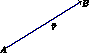
\includegraphics[scale=3.0]{vector.pdf}
   \caption{A Vector}
   \label{fig:figure-1-vector}
\end{figure}


\begin{eg}[Examples of vectors]
  Here are some important examples of vectors\\
  \vspace{-10px}
  \begin{itemize}
    \item The displacement of a particle is a vector.
    \item The velocity of a particle is a vector.
    \item The force acting on a particle is a vector.
  \end{itemize}

\end{eg}

\begin{notation}
  Vectors can be denoted in 3 ways,
  \begin{itemize}
    \item Using {\bf boldface notation}: $\boldsymbol{V}$
    \item Underlining:  $\underline{V}$ 
    \item An arrow over the symbol: $\vec{V}$

  \end{itemize}


\end{notation}

\section{Euclidean Three Space $\mathbb{E}^3$}

\begin{definition}[Euclidian Three Space]
 
  Euclidean Three Space is the set of all ordered triples of real numbers.\\
  \vspace{-10px}
  \begin{equation}
    \mathbb{E}^3 = \{(x,y,z) | x,y,z \in \mathbb{R}\}
  \end{equation}

\end{definition}

The \textbf{axes} of $\mathbb{E}^{3}$ are the $x$, $y$ and $z$, i.e.
\vspace{-10px}
\begin{equation}
  x = (x,0,0), y = (0,y,0), z = (0,0,z)
\end{equation}

We orient the axis according to the \textbf{right hand rule}. This is shown in the following diagram:

%generate tikz code for axes in 3d space

\begin{figure}[H]
  \centering
  \begin{tikzpicture}
    \draw[->] (0,0,0) -- (3,0,0) node[anchor=north east]{$y$};
    \draw[->] (0,0,0) -- (0,3,0) node[anchor=north west]{$z$};
    \draw[->] (0,0,0) -- (0,0,3) node[anchor=south]{$x$};
  \end{tikzpicture}
  \caption{Axes in $\mathbb{E}^3$}
\end{figure}

\begin{note}
  We need to pick an \textbf{origin} and stay with it. We will use the origin $(0,0,0)$.
\end{note} 

\section{Vectors in $\mathbb{E}^3$}
\subsection{Distance in $\mathbb{E}^3$}
Let $P$ and $P^{'}$ be points in $\mathbb{E}^3$. And let $P = (x,y,z)$ and $P^{'} = (x^{'},y^{'},z^{'})$.
\begin{definition}[Distance in $\mathbb{E}^3$]
  The \textbf{distance} between $P$ and $P^{'}$ is defined as:
  \begin{equation}
    d(P,P^{'}) = \sqrt{(x-x^{'})^2 + (y-y^{'})^2 + (z-z^{'})^2}
  \end{equation}
\end{definition}
This is illustrated in the following diagram
\begin{figure}[H]
\centering
   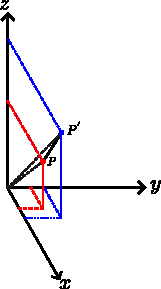
\includegraphics[scale=1.75]{distance.pdf}
   \caption{Distance in $\mathbb{E}^3$}
   \label{fig:figure-8-space}
\end{figure}
\clearpage
\subsection{Vectors in $\mathbb{E}^3$}
\begin{definition}[Vectors in $\mathbb{E}^3$]
  A \textbf{vector} in $\mathbb{E}^3$ is an ordered triple of real numbers.\\
  \vspace{-10px}
  \begin{equation}
    \vec{v} = (v_1,v_2,v_3)
  \end{equation}
\end{definition}

\begin{notation}
  We can also represent vectors using {\bf column notation}
  $$\underline{v} = \begin{bmatrix} v_1 \\ v_2 \\ v_3\end{bmatrix} $$
  
\end{notation}


% \section{Vector Algebra}

\subsection{Vector Magnitude}

\begin{definition}[Vector Magnitude]
  Let $\vec{v} = (v_1, v_2, v_3)$ be a vector in $\mathbb{E}^3$. The \textbf{magnitude} of $\vec{v}$ is defined as:
  \begin{equation}
    \|\vec{v}\| = \sqrt{v_1^2 + v_2^2 + v_3^2}
  \end{equation}
\end{definition}

\subsection{Vector Addition}

\begin{definition}[Vector Addition]
  Let $\vec{v} = (v_1, v_2, v_3)$ and $\vec{w} = (w_1, w_2, w_3)$ be vectors in $\mathbb{E}^3$. The \textbf{sum} of $\vec{v}$ and $\vec{w}$ is defined as:
  \begin{equation}
    \vec{v} + \vec{w} = (v_1 + w_1, v_2 + w_2, v_3 + w_3)
  \end{equation}
\end{definition}

Geometrically this can be seen as the {\bf diagonal} of a paralleleogram. Geometrically it is clear that you get the same effect as travelling along $\vec{v}$ and then $\vec{u}$

\begin{figure}[H]
\centering
   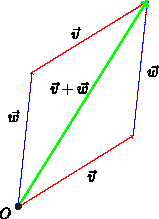
\includegraphics[scale=2.0]{vector_addition.pdf}
   \caption{Vector Addition} 
   \label{fig:figure-2-vector-addition}
\end{figure}

\clearpage

\subsubsection*{Vector Addition Properties}
\vspace{5px}
 
\begin{theorem}[Commutativity]
Suppose $\vec{v}$ and $\vec{w}$ be vectors in $\mathbb{E}^3$.\\
  If $\vec{v} = \left( v_1, v_2, v_3 \right)$ and $\vec{w} = \left(w_1, w_2, w_3 \right)$ be vectors in $\mathbb{E}^{3}$, then
  \begin{equation}
      \vec{v} + \vec{w} = \vec{w} + \vec{v}    
  \end{equation}
\end{theorem}
\begin{proof}
  
\end{proof}


% \section{Standard Basis}
Standard basis vectors are also known as standard {\bf unit vectors}. These are used to represent vectors in $\mathbb{E}^3$

\begin{definition}
  The standard basis vectors are defined as follows:
  \begin{align*}
    \hat{i} &= (1, 0, 0 ) \\
    \hat{j} &=  (0, 1, 0) \\
    \hat{k} &=  (0, 0, 1)
  \end{align*}
such that $\mid \hat{i} \mid = \mid \hat{j} \mid = \mid \hat{k} \mid.$ 
\end{definition}

Any vector can be represented using standard basis vectors. 

Suppose you are a given a vector $\vec{v} = (v_1, v_2, v_3)$. This can be represented as follows:
\begin{equation}
  \vec{v} = \begin{bmatrix} v_1 \\ v_2 \\ v_3 \end{bmatrix}  =v_1\hat{i} + v_2\hat{j} + v_3\hat{k}
\end{equation}

\begin{eg}
  Let $\vec{v} = (2, 3, 4)$. Then, 
  \begin{align*}
    \vec{v} &= 2\hat{i} + 3\hat{j} + 4\hat{k} \\
    &= 2(1, 0, 0) + 3(0, 1, 0) + 4(0, 0, 1) \\
    &= (2, 0, 0) + (0, 3, 0) + (0, 0, 4) \\
    &= (2, 3, 4)
  \end{align*}
\end{eg}


\begin{figure}[H]
\centering
   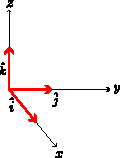
\includegraphics[scale=2.5]{standard-basis.pdf}
   \caption{Standard Basis Vectors}
   \label{fig:figure-3-unit-vector}
\end{figure}

\subsubsection{Algebra with Standard Basis Vectors}
\vspace{5px}
\begin{eg}
  Let $\vec{v}$ and $\vec{w} \in \mathbb{E}^3$ 
  \begin{flalign*}
    \vec{v} \pm \vec{w} = \begin{bmatrix} v_1 \pm w_1 \\ v_2 \pm w_2 \\ v_3 \pm w_3\end{bmatrix}  = (v_1 \pm w_1)\hat{i} + (v_2 \pm w_2)\hat{j} + (v_3 \pm w_3)\hat{k} &
  \end{flalign*}
\end{eg}


\begin{eg}
  Let $\vec{v}$ and $\vec{w} \in \mathbb{E}^3$ 
  \begin{flalign*}
    \lambda\vec{v} = \begin{bmatrix} \lambda v_1 \\ \lambda v_2 \\ \lambda v_3\end{bmatrix}  = (\lambda v_1)\hat{i} + (\lambda v_2)\hat{j} + (\lambda v_3)\hat{k} &
  \end{flalign*}
\end{eg}

\begin{note}
 The 0 vector is:
  $$\underline{0} = \begin{bmatrix} 0 \\ 0 \\ 0 \end{bmatrix} = 0\hat{i} + 0\hat{j} + 0\hat{k}$$
Any vector $\vec{v} \in \mathbb{E}^3$ added to the 0 vector is itself:
$$\vec{v} + \underline{0} = \vec{v}$$
\end{note}

Here is an example of algebra with standard basis vectors:
\begin{eg}
  Let $\vec{v} = (2, 3, 4)$ and $\vec{w} = (1, 2, 3)$. Then,
  \begin{align*}
    \vec{v} + \vec{w} &= (2, 3, 4) + (1, 2, 3) \\
    &= (2 + 1, 3 + 2, 4 + 3) \\
    &= (3, 5, 7)
  \end{align*}
\end{eg}

\subsubsection{Alternate Notation for Standard Basis Vectors}
\vspace{5px}
\begin{notation}
  We can change notation for standard basis vectors as follows:
  $$\hat{i} = \vec{e}_{1} \ \ \ \ \ \ \ \ \hat{j} = \vec{e}_{2} \ \ \ \ \ \ \ \ \hat{k} = \vec{e}_{3}$$
\end{notation}
and therefore we can write:
$$\vec{v} = v_1\hat{i} + v_2\hat{j} + v_3\hat{k} = \sum^{3}_{a=1}v_a \vec{e}_a$$

% \section{Position Vectors}

\begin{definition}
  A {\bf position vector} is a vector that represents the position of a point in space relative to the origin, $O$. 
\end{definition}

Let any vector $\vec{v}$ be the position vector of a point $P$ in space. Then, the coordinates of $P$ are given by the components of $\vec{v}$:
\begin{figure}[H]
\centering
   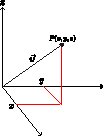
\includegraphics[scale=2.5]{position-vectors.pdf}
   \caption{Position Vector}
   \label{fig:figure-4-position-vector}
\end{figure}

So the position vector of $P$ is given by:
\begin{equation}
  \vec{v} = \begin{bmatrix} x \\ y \\ j \end{bmatrix}  =x\hat{i} + y\hat{j} + k\hat{k}
\end{equation}
\clearpage

% \section{Scalar Product}

Scalar product is also known as dot product, is a function denoted by $\cdot$:
$$\cdot: \mathbb{E}^3 \times \mathbb{E}^3 \mapsto \mathbb{R}$$
i.e. it takes two vectors and returns a scalar.

\begin{definition}[Planar Angle]
  Let $\vec{v}$ and $\vec{w}$ be two vectors in $\mathbb{E}^3$ and $\theta \in \mathbb{R}$.
  \newline \newline
  The {\bf planar angle} between two vectors $\vec{v}$ and $\vec{w}$ is the angle $\theta$ between them in the plane spanned by $\vec{v}$ and $\vec{w}$.
  
  \begin{figure}[H]
    \centering
    \tikzset{every picture/.style={line width=0.75pt}} %set default line width to 0.75pt        

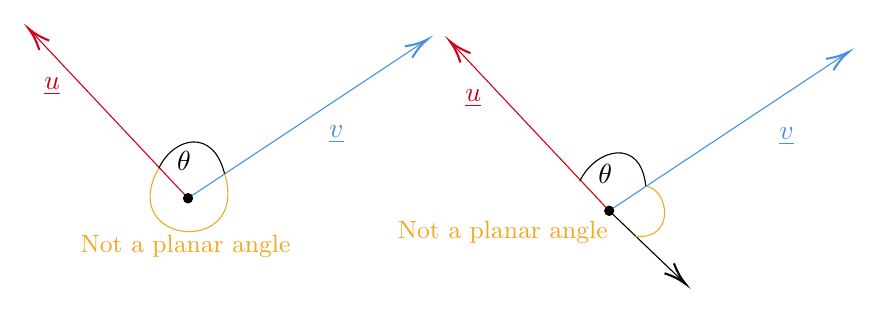
\begin{tikzpicture}[x=0.75pt,y=0.75pt,yscale=-1,xscale=1]
%uncomment if require: \path (0,402); %set diagram left start at 0, and has height of 402

%Straight Lines [id:da4437652617379132] 
\draw [color={rgb, 255:red, 208; green, 2; blue, 27 }  ,draw opacity=1 ]   (184.85,216.98) -- (109.47,136.76) ;
\draw [shift={(108.1,135.3)}, rotate = 46.79] [color={rgb, 255:red, 208; green, 2; blue, 27 }  ,draw opacity=1 ][line width=0.75]    (10.93,-3.29) .. controls (6.95,-1.4) and (3.31,-0.3) .. (0,0) .. controls (3.31,0.3) and (6.95,1.4) .. (10.93,3.29)   ;
%Straight Lines [id:da6919359366246228] 
\draw [color={rgb, 255:red, 74; green, 144; blue, 226 }  ,draw opacity=1 ]   (184.85,216.98) -- (298.51,141.58) ;
\draw [shift={(300.17,140.48)}, rotate = 146.44] [color={rgb, 255:red, 74; green, 144; blue, 226 }  ,draw opacity=1 ][line width=0.75]    (10.93,-3.29) .. controls (6.95,-1.4) and (3.31,-0.3) .. (0,0) .. controls (3.31,0.3) and (6.95,1.4) .. (10.93,3.29)   ;
%Shape: Ellipse [id:dp7599712014506931] 
\draw  [fill={rgb, 255:red, 0; green, 0; blue, 0 }  ,fill opacity=1 ] (182.67,216.98) .. controls (182.67,218.22) and (183.65,219.23) .. (184.85,219.23) .. controls (186.04,219.23) and (187.02,218.22) .. (187.02,216.98) .. controls (187.02,215.75) and (186.04,214.74) .. (184.85,214.74) .. controls (183.65,214.74) and (182.67,215.75) .. (182.67,216.98) -- cycle ;
%Curve Lines [id:da9435159136782311] 
\draw    (170.73,202.58) .. controls (178.25,187.05) and (197.1,183.3) .. (202.47,205.17) ;
%Curve Lines [id:da043732572464616704] 
\draw [color={rgb, 255:red, 245; green, 166; blue, 35 }  ,draw opacity=1 ]   (170.73,202.58) .. controls (149.85,239.67) and (214.99,245.71) .. (202.47,205.17) ;
%Straight Lines [id:da6201503651143601] 
\draw [color={rgb, 255:red, 208; green, 2; blue, 27 }  ,draw opacity=1 ]   (387.77,223.02) -- (312.4,142.8) ;
\draw [shift={(311.03,141.34)}, rotate = 46.79] [color={rgb, 255:red, 208; green, 2; blue, 27 }  ,draw opacity=1 ][line width=0.75]    (10.93,-3.29) .. controls (6.95,-1.4) and (3.31,-0.3) .. (0,0) .. controls (3.31,0.3) and (6.95,1.4) .. (10.93,3.29)   ;
%Straight Lines [id:da44499435743744065] 
\draw [color={rgb, 255:red, 74; green, 144; blue, 226 }  ,draw opacity=1 ]   (387.77,223.02) -- (501.43,147.62) ;
\draw [shift={(503.1,146.51)}, rotate = 146.44] [color={rgb, 255:red, 74; green, 144; blue, 226 }  ,draw opacity=1 ][line width=0.75]    (10.93,-3.29) .. controls (6.95,-1.4) and (3.31,-0.3) .. (0,0) .. controls (3.31,0.3) and (6.95,1.4) .. (10.93,3.29)   ;
%Shape: Ellipse [id:dp13145555074263104] 
\draw  [fill={rgb, 255:red, 0; green, 0; blue, 0 }  ,fill opacity=1 ] (385.6,223.02) .. controls (385.6,224.26) and (386.57,225.26) .. (387.77,225.26) .. controls (388.97,225.26) and (389.94,224.26) .. (389.94,223.02) .. controls (389.94,221.78) and (388.97,220.78) .. (387.77,220.78) .. controls (386.57,220.78) and (385.6,221.78) .. (385.6,223.02) -- cycle ;
%Curve Lines [id:da424029835736604] 
\draw    (373.66,208.62) .. controls (381.18,193.09) and (403.1,187.3) .. (405.39,211.2) ;
%Straight Lines [id:da38053982821885624] 
\draw    (387.77,223.02) -- (423.16,256.92) ;
\draw [shift={(424.6,258.3)}, rotate = 223.77] [color={rgb, 255:red, 0; green, 0; blue, 0 }  ][line width=0.75]    (10.93,-3.29) .. controls (6.95,-1.4) and (3.31,-0.3) .. (0,0) .. controls (3.31,0.3) and (6.95,1.4) .. (10.93,3.29)   ;
%Curve Lines [id:da7344761482411821] 
\draw [color={rgb, 255:red, 245; green, 166; blue, 35 }  ,draw opacity=1 ]   (405.39,211.2) .. controls (416.25,212.07) and (420.43,237.08) .. (400.38,235.36) ;

% Text Node
\draw (114.3,157.54) node [anchor=north west][inner sep=0.75pt]  [color={rgb, 255:red, 208; green, 2; blue, 27 }  ,opacity=1 ] [align=left] {$\displaystyle \underline{u}$};
% Text Node
\draw (251.61,180.86) node [anchor=north west][inner sep=0.75pt]  [color={rgb, 255:red, 74; green, 144; blue, 226 }  ,opacity=1 ] [align=left] {$\displaystyle \underline{v}$};
% Text Node
\draw (178.35,193.32) node [anchor=north west][inner sep=0.75pt]   [align=left] {$\displaystyle \theta $};
% Text Node
\draw (131.86,233.65) node [anchor=north west][inner sep=0.75pt]  [font=\small,color={rgb, 255:red, 245; green, 166; blue, 35 }  ,opacity=1 ] [align=left] {Not a planar angle};
% Text Node
\draw (317.22,163.58) node [anchor=north west][inner sep=0.75pt]  [color={rgb, 255:red, 208; green, 2; blue, 27 }  ,opacity=1 ] [align=left] {$\displaystyle \underline{u}$};
% Text Node
\draw (468.54,181.89) node [anchor=north west][inner sep=0.75pt]  [color={rgb, 255:red, 74; green, 144; blue, 226 }  ,opacity=1 ] [align=left] {$\displaystyle \underline{v}$};
% Text Node
\draw (381.28,199.36) node [anchor=north west][inner sep=0.75pt]   [align=left] {$\displaystyle \theta $};
% Text Node
\draw (284.68,226.75) node [anchor=north west][inner sep=0.75pt]  [font=\small,color={rgb, 255:red, 245; green, 166; blue, 35 }  ,opacity=1 ] [align=left] {Not a planar angle};

\end{tikzpicture}
\end{figure}

Choose the planar angle $\theta$ such that 
$$0 \leq \theta \leq \pi$$.
\end{definition}


\begin{definition}[Scalar Product]

  Let $\vec{v}$ and $\vec{w}$ be two vectors in $\mathbb{E}^3$ and $\theta \in \mathbb{R}$ be the planar angle between them. \\ 
Then, the scalar product of $\vec{v}$ and $\vec{w}$ is defined as:
  \begin{equation}
    \vec{v} \cdot \vec{w} = \mid \vec{v} \mid \mid \vec{w} \mid \cos \theta
  \end{equation}
\end{definition}

\begin{note}
  Two vectors do not lie in the same line, always in the same plane.
  By the convention, the angle $\theta \in [0,\pi] \Rightarrow 0 \leq \theta \leq \pi$.
\end{note}

\subsection{Properties of Scalar Product}
\begin{theorem}[Commutative]
Let $\vec{v}$ and $\vec{w}$ be two vectors in $\mathbb{E}^3$. Then,
  \begin{equation}
    \vec{v} \cdot \vec{w} = \vec{w} \cdot \vec{v}
  \end{equation}
\end{theorem}
\begin{proof}
Since the planar angle $\theta$ is the same for both $\vec{v}$ and $\vec{w}$,
\begin{align*}
  \vec{v} \cdot \vec{w} &= \mid \vec{v} \mid \mid \vec{w} \mid \cos \theta \\
  &= \mid \vec{w} \mid \mid \vec{v} \mid \cos \theta \\
  &= \vec{w} \cdot \vec{v}  
\end{align*}
\end{proof}
\begin{theorem}[Orthogonal Vectors]
 Let $\vec{v}$ and $\vec{w}$ be two vectors in $\mathbb{E}^3$. Then,
  \begin{equation}
    \vec{v} \cdot \vec{w} = 0 \iff \vec{v} \perp \vec{w}
  \end{equation} 
\end{theorem}
\begin{proof}
When $\vec{v} \perp \vec{w}$, the planar angle $\theta = \frac{\pi}{2}$. 
Therefore, 
\begin{align*}
  \vec{v} \cdot \vec{w} &= \mid \vec{v} \mid \mid \vec{w} \mid \cos \theta \\
  &= \mid \vec{v} \mid \mid \vec{w} \mid \cos \frac{\pi}{2} \\
  &= \mid \vec{v} \mid \mid \vec{w} \mid \cdot 0 \\
  &= 0
\end{align*}
  i.e. $\vec{v}$ and $\vec{w}$ are orthogonal.
\end{proof}

\begin{theorem}[Distributivity over scalar multiplication]
  Let $\vec{v}, \vec{w} \in \mathbb{E}^3$ and $\lambda \in \mathbb{R}$. Then,
  \begin{equation}
    \lambda(\vec{v} \cdot \vec{w}) = (\lambda \vec{v}) \cdot \vec{w} = \vec{v} \cdot (\lambda \vec{w})
  \end{equation}
\end{theorem}

\begin{theorem}[Distributivity over Addition]
  Let $\vec{u}, \vec{v}, \vec{w} \in \mathbb{E}^3$. Then,
  \begin{equation}
    \vec{u} \cdot (\vec{v} + \vec{w}) = \vec{u} \cdot \vec{v} + \vec{u} \cdot \vec{w}
  \end{equation}
\end{theorem}

\begin{note}
  Properties of scalar product for standard basis vectors:
  \begin{align*}
    \hat{i} \cdot \hat{i} &= 1 \\
    \hat{j} \cdot \hat{j} &= 1 \\
    \hat{k} \cdot \hat{k} &= 1 \\
    \hat{i} \cdot \hat{j} &= 0 \\
    \hat{i} \cdot \hat{k} &= 0 \\
    \hat{j} \cdot \hat{k} &= 0 \\
  \end{align*}
\end{note}

\subsection{Scalar Product in terms of Components}
\vspace{5px}
\begin{theorem}
  Let $\vec{v} = (v_1, v_2, v_3)$ and $\vec{w} = (w_1, w_2, w_3)$ be two vectors in $\mathbb{E}^3$. Then,
  \begin{equation}
    \vec{v} \cdot \vec{w} = \sum_{i=1}^{3}v_{i}w_{i} = v_1w_1 + v_2w_2 + v_3w_3
  \end{equation}
\end{theorem}
\begin{proof}
  Let $\vec{v}, \vec{w} \in \mathbb{E}^{3}$. Then, 
  \begin{flalign*}
    \vec{v} \cdot \vec{w} &= (v_1 \hat{i} + v_2 \hat{j} + v_3 \hat{k}) \cdot (w_1 \hat{i} + w_2 \hat{j} + w_3 \hat{k}) &\\ \\ 
      &= v_{1} \cdot (w_{1} \hat{i} + w_{2}\hat{j} + w_3 \hat{k}) + v_{2} \cdot (w_{1} \hat{i} + w_{2}\hat{j} + w_3 \hat{k}) + v_{3} \cdot (w_{1} \hat{i} + w_{2}\hat{j} + w_3 \hat{k})   &\\ \\
      &= v_{1}w_{1} \hat{i} \cdot \hat{i} + \cancel{v_{1}w_{2} \hat{i} \cdot \hat{j}} + \cancel{v_{1}w_{3} \hat{i} \cdot \hat{k}}  + \cancel{v_{2}w_{1} \hat{j} \cdot \hat{i}} + v_{2}w_{2} \hat{j} \cdot \hat{j} + \cancel{v_{2}w_{3} \hat{j} \cdot \hat{k}} \\  &+ \cancel{v_{3}w_{1} \hat{k} \cdot \hat{i}} + \cancel{v_{3}w_{2} \hat{k} \cdot \hat{j}} + v_{3}w_{3} \hat{k} \cdot \hat{k} &\\ \\
      &= v_{1}w_{1} + v_{2}w_{2} + v_{3}w_{3} &\\ \\ 
      &= \sum_{i=1}^{3}v_{i}w_{i} = v_1w_1 + v_2w_2 + v_3w_3
  \end{flalign*}
\end{proof}

\subsection{Using Scalar Product to find the length of a vector}
We can also use scalar product to find the length of a vector.
\begin{theorem}
  Let $\vec{v} \in \mathbb{E}^3$. Then,
  \begin{equation}
    \mid \vec{v} \mid = \sqrt{\vec{v} \cdot \vec{v}}
  \end{equation}
\end{theorem}
\begin{proof}
Let $\vec{v} \in \mathbb{E}^3$. Then,
  \begin{flalign*}
    \mid \vec{v} \mid &= \sqrt{v_1^{2} + v_2^{2} + v_3^{2}} \\ \\ 
    &= \sqrt{v_1v_1 + v_2v_2 + v_3v_3}  \\ \\
    &= \sqrt{\vec{v} \cdot \vec{v}}  
  \end{flalign*}
\end{proof}

\subsection{Using Scalar Product to find the angle between two vectors}

\begin{theorem}
  Let $\vec{v}, \vec{w} \in \mathbb{E}^3$. Then, the planar angle $\theta$ between $\vec{v}$ and $\vec{w}$ is given by:
  \begin{equation}
    \theta = \cos^{-1} \left( \frac{\vec{v} \cdot \vec{w}}{\mid \vec{v} \mid \mid \vec{w} \mid} \right)
  \end{equation}
\end{theorem}
\begin{proof}
  Let $\vec{v}, \vec{w} \in \mathbb{E}^3$. Then,
  \begin{flalign*}
    \vec{v} \cdot \vec{w} &= \mid \vec{v} \mid \mid \vec{w} \mid \cos \theta  \\ \\
    &= v_1w_1 + v_2w_2 + v_3w_3 \\ \\
    \Rightarrow \cos \theta &= \frac{v_1w_1 + v_2w_2 + v_3w_3}{\mid \vec{v} \mid \mid \vec{w} \mid} \\ \\
    \Rightarrow \theta &= \cos^{-1} \left( \frac{\vec{v} \cdot \vec{w}}{\mid \vec{v} \mid \mid \vec{w} \mid} \right)
  \end{flalign*}
\end{proof}

\begin{note}
  Some basic properties of scalar product:
  \begin{enumerate}
    \item If $\vec{v} \cdot \vec{w} = 0$, then $\theta = \frac{\pi}{2}$.
    \item If $\vec{v} \cdot \vec{w} > 0$, then $\theta \in [0, \frac{\pi}{2})$.
    \item If $\vec{v} \cdot \vec{w} < 0$, then $\theta \in (\frac{\pi}{2}, \pi]$.
  \end{enumerate}
\end{note}

% \section{Cross Product}

% \section{Kronecker-Delta}

As shown before, the properties of the {\bf scalar product}, the {\bf orthonormal basis} vectors have the following properties
$$\underline{e_{1}} \cdot \underline{e_{2}}= 0 = \underline{e_{1}} \cdot \underline{e_{3}} = \underline{e_{2}} \cdot \underline{e_{3}}$$
and
$$\underline{e_{1}} \cdot \underline{e_{1}}= 1 = \underline{e_{2}} \cdot \underline{e_{2}} = \underline{e_{3}} \cdot \underline{e_{3}}$$
We can abbreviate the definition using the {\bf Kronecker-Delta}

\begin{definition}[Kronecker-Delta]

	Let $a,b \in {1,2,3}$. Then we can write:

	\begin{equation}
		\label{eq:kronecker-delta}
		\underline{e_{a}}\cdot \underline{e_{b}}
		=
		\begin{cases}
			1 \ \ \text{if } a = b = 1,2,3 \\
			0  \ \ \text{if } a \neq b
		\end{cases}
		= \delta_{ab}
	\end{equation}

	This will also be useful for calculating scalar product
\end{definition}

\subsection{Scalar product using Kronecker-Delta}
\begin{theorem}[Scalar Product using Kroncker-Delta]
	Let $\vec{a} \vec{b} \in \mathbb{E}^3$. Then
	\begin{equation}
		\vec{a} \cdot \vec{v} = \sum_{i=1}^{3}a_kb_k
	\end{equation}
\end{theorem}
\begin{proof}
	\begin{align*}
		\underline{a} \ \cdot \ \underline{b} & = \Big( \sum\limits_{k = 1}^{3}a_k\underline{e_{k}} \Big)\ \cdot \ \Big( \sum\limits_{l = 1}^{3}b_l\underline{e_{l}} \Big) \\ \\
		                                      & = \sum_{k, \ l} a_{k} \ b_{l} \ \underline{e_{k}}\ \cdot \ \underline{e_{l}}                                               \\ \\
		                                      & = \sum_{k, \ l} a_{k} \ b_{l} \ \delta_{kl}
	\end{align*}
	Now by the definition of Kronecker-Delta \ref{eq:kronecker-delta}, it is 0 for all cases except when $k = l$. where it has a value of {\bf 1} So the summation becomes:
	$$\underline{a} \ \cdot \underline{b} =\sum_{k=1}^{3} a_{k} \ b_{k}$$
\end{proof}

% \section{Levi-Civita}
We can represent the cross product using {\bf Levi-Civita Symbol}

\begin{definition}[Levi-Civita]
	Let $a, b, c \in {1,2,3}$. Then we write:
	\begin{equation}
		\label{eq:levi-civita}
		\varepsilon_{abc}
		=
		\begin{cases}
			0  \ \ \ \ \  \text{if } \space a = b = c  \space \space \text{ or more generally} \space a,b,c \space \text{is {\bf not} permutation of } \space 1,2,3 \\
			+1  \ \ \ \ \  \text{if } \space a,b,c \space \text{ is an {\bf even} permuation of } \space 1,2,3                                                      \\
			-1  \ \ \ \ \ \text{if } \space a,b,c \space \text{ is an {\bf odd} permuation of } \space 1,2,3
		\end{cases}
	\end{equation}
\end{definition}

\begin{note}
	Value of $\varepsilon_{abc}$ depends on the {\bf parity} of the permutatiom.
\end{note}

\subsection{Cross product of Orthonoarmal Basis Using Levi-Civita}
\begin{definition}
	Then we can write the cross product {\bf Orthonoarmal Basis Vectors} $\underline{e_1}, \underline{e_2}, \underline{e_3}$ in the following way
	\begin{equation}
		\label{eq: levi-orthonormal}
		\underline{e_a} \times \underline{e_b} = \sum_{i=1}^{3}a_{k}b_{k}\varepsilon_{abc}
	\end{equation}

\end{definition}

\subsection{Cross Product of Vectors in Levi-Civita Notation}
\begin{theorem}[Cross Product using Levi-Civita Notation]
	Let $\vec{a}, \vec{b} \in \mathbb{E}^3$. Then
	\begin{equation}
		\label{eq:levi-civita-cross-product}
		\vec{a} \times \vec{b} = \sum_{m=1}^{3}(\vec{a} \times \vec{b})_{m}\underline{e_m}
	\end{equation}
	where $(\vec{a} \times \vec{b})_m$ is the {\bf mth component}
	\begin{equation}
		\label{eq: mth-component}
		(\vec{a} \times \vec{b})_m = \sum_{k, \ l}\varepsilon_{abc}a_{k}b_{l}
	\end{equation}
\end{theorem}
\begin{proof}
	Let
	$$
		\underline{a} = a_{k}\underline{e_{k}} = \sum_{k=1}^{3}a_{k}\ \underline{e_{k}} \hspace{100px} \underline{b} = b_{l}\underline{e_{l}}= \sum\limits_{l=1}^{3} b_{l}\ \underline{e_{l}}
	$$
	Observe the use of {\bf Eintein's Notation} (see below) and observe that
	\begin{align*}
		\underline{a} \times \underline{b} & = \Big( \sum\limits_{k = 1}^{3}a_k\underline{e_{k}} \Big)\ \times \ \Big( \sum\limits_{l = 1}^{3}b_l\underline{e_{l}} \Big) \\ \\
		                                   & = \sum\limits_{k, \ l}a_{k} \ b_{k} \ \underline{e_{k}} \times \underline{e_{l}}
	\end{align*}
	And therefore by \ref{eq: levi-orthonormal}, we can rewrite it in the following way
	$$\hspace{-80px} = \sum\limits_{k,\ l,\ m} a_{k} \ b_{l} \ \epsilon_{klm} \ \underline{e_m}$$
	Define the {\bf mth component} as
	$$(\vec{a} \times \vec{b})_m =  \sum_{k, \ l}\varepsilon_{abc}a_{k}b_{l}$$
	and hence we get \ref{eq:levi-civita-cross-product}
\end{proof}

% \section{Einstein's Notation}

\begin{definition}[Einstein's Notation]

	If {\bf two} indicies are {\bf repeated}, then they are {\bf summed} and we can {\bf suppress} the summation
\end{definition}

\subsection{Scalar Product using Einstein Convention}
\begin{eg}
	$$\sum_{i=1}^{3}a_{k}b_{k} = a_{k}b_{k}$$
	Here the {\bf repeated index} is $k$
\end{eg}

\subsection{Cross Product using Einstein Convention}
\begin{eg}
	Here the {\bf repeated index} is $k$ and $l$
	$$(a \ \times\ b)_{m}= \sum\limits_{k,\  l}^{3}\epsilon_{klm}a_{k}\ b_k =\epsilon_{klm} a_{k} \ b_{k}$$

\end{eg}

% \section{Triple Scalar Product}

\begin{theorem}[Triple Scalar Product]
	Let $\vec{a}, \vec{b}, \vec{c} \in \mathbb{E}^{3}$. Then
	\begin{equation}
		\label{eq: triple-scalar-product}
		\vec{a} \cdot (\vec{b} \times \vec{c}) = \varepsilon_{abc}a_pb_qc_r
	\end{equation}
\end{theorem}
\begin{note}
	We have used \textbf{Einstein's Notation} for Scalar and Vector Product as well as Levi-Civita Notation \ref{eq:levi-civita}
\end{note}
\begin{proof}
	\begin{align*} \underline{a} \ \cdot \ (\underline{b} \times \underline{c}) & = a_{p}\ (\underline{b} \times \underline{c})_{p} \\ \\ &= a_{p}\ \epsilon_{pqr}\ b_{q}\ c_{r}\\ \\
                                                                            & = \epsilon_{pqr}\ a_{p}\ b_{q}\ c_{r}\end{align*}
\end{proof}
\begin{note}
	Although not mathematically valid, we can use the {\bf determinant method}
	$$\underline{a} \cdot(\underline{b} \times \underline{c}) =
		\det\begin{pmatrix}a_1 & a_2 & a_3 \\ b_{1} & b_{2} & b_{3} \\ c_{1}  & c_{2} & c_{3}\end{pmatrix}$$
\end{note}

% \section{Useful Properties of Kronecker-Delta and Levi-Civita}
\begin{theorem}
	\begin{equation}
		\label{eq: levi-kronecker-property-1}
		\epsilon_{pqr}\epsilon_{ruv} = (\delta_{pu}\delta_{qv} - \delta_{pv}\delta_{qu})
	\end{equation}
\end{theorem}
\begin{note}
	These are useful identity/trick to remember (remeber the use of {\bf Einstein's Notation})
	$$\delta_{aa} = \delta_{11} + \delta_{22} + \delta_{33} = 3$$
	\\
	\begin{equation*}
		\delta_{ab}\delta_{bc}=\delta_{a1}\delta_{1c} + \delta_{a2}\delta_{2c} + \delta_{a3}\delta_{3c}
		= \begin{cases}
			1 & \text{if } a = c    \\
			0 & \text{if } a \neq c
		\end{cases}
		\ \ \ = \delta_{ac}
	\end{equation*}
\end{note}


\section{Triple Vector Product}
\begin{theorem}[Triple Vector Product]
	Let $\underline{a}, \underline{b}, \underline{c} \in \mathbb{E}^3$
	\begin{equation}
		\label{eq: triple-vector-product}
		\underline{a} \times (\underline{b} \times \underline{c}) = \underline{b}(\underline{a} \cdot \underline{c}) - \underline{c}(\underline{a} \cdot \underline{b})
	\end{equation}
\end{theorem}
\begin{proof}
	Taking three vectors $\underline{a}, \underline{b} \text{ and } \underline{c}$, we {\em calculate} the \textbf{pth component} first:
	\begin{align*}
		[\underline{a} \times (\underline{b} \times \underline{c})]_{p} & = \epsilon_{pqr}\ a_{q}(\underline{b} \times \underline{c})_{r} \\ \\
		                                                                & = \epsilon_{pqr}\ a_{q} \ \epsilon_{ruv}\ b_{u}\ c_{v}
	\end{align*}
	using identity \ref{eq: levi-kronecker-property-1}, we get
	\begin{align*}
		[\underline{a} \times (\underline{b} \times \underline{c})]_{p} & = (\delta_{pu}\delta_{qv} - \delta_{pv}\delta_{qu})a_{q}b_{u}c_{v}
	\end{align*}
	Use the explanation below for completion
\end{proof}

\begin{figure}[H]
	\centering
	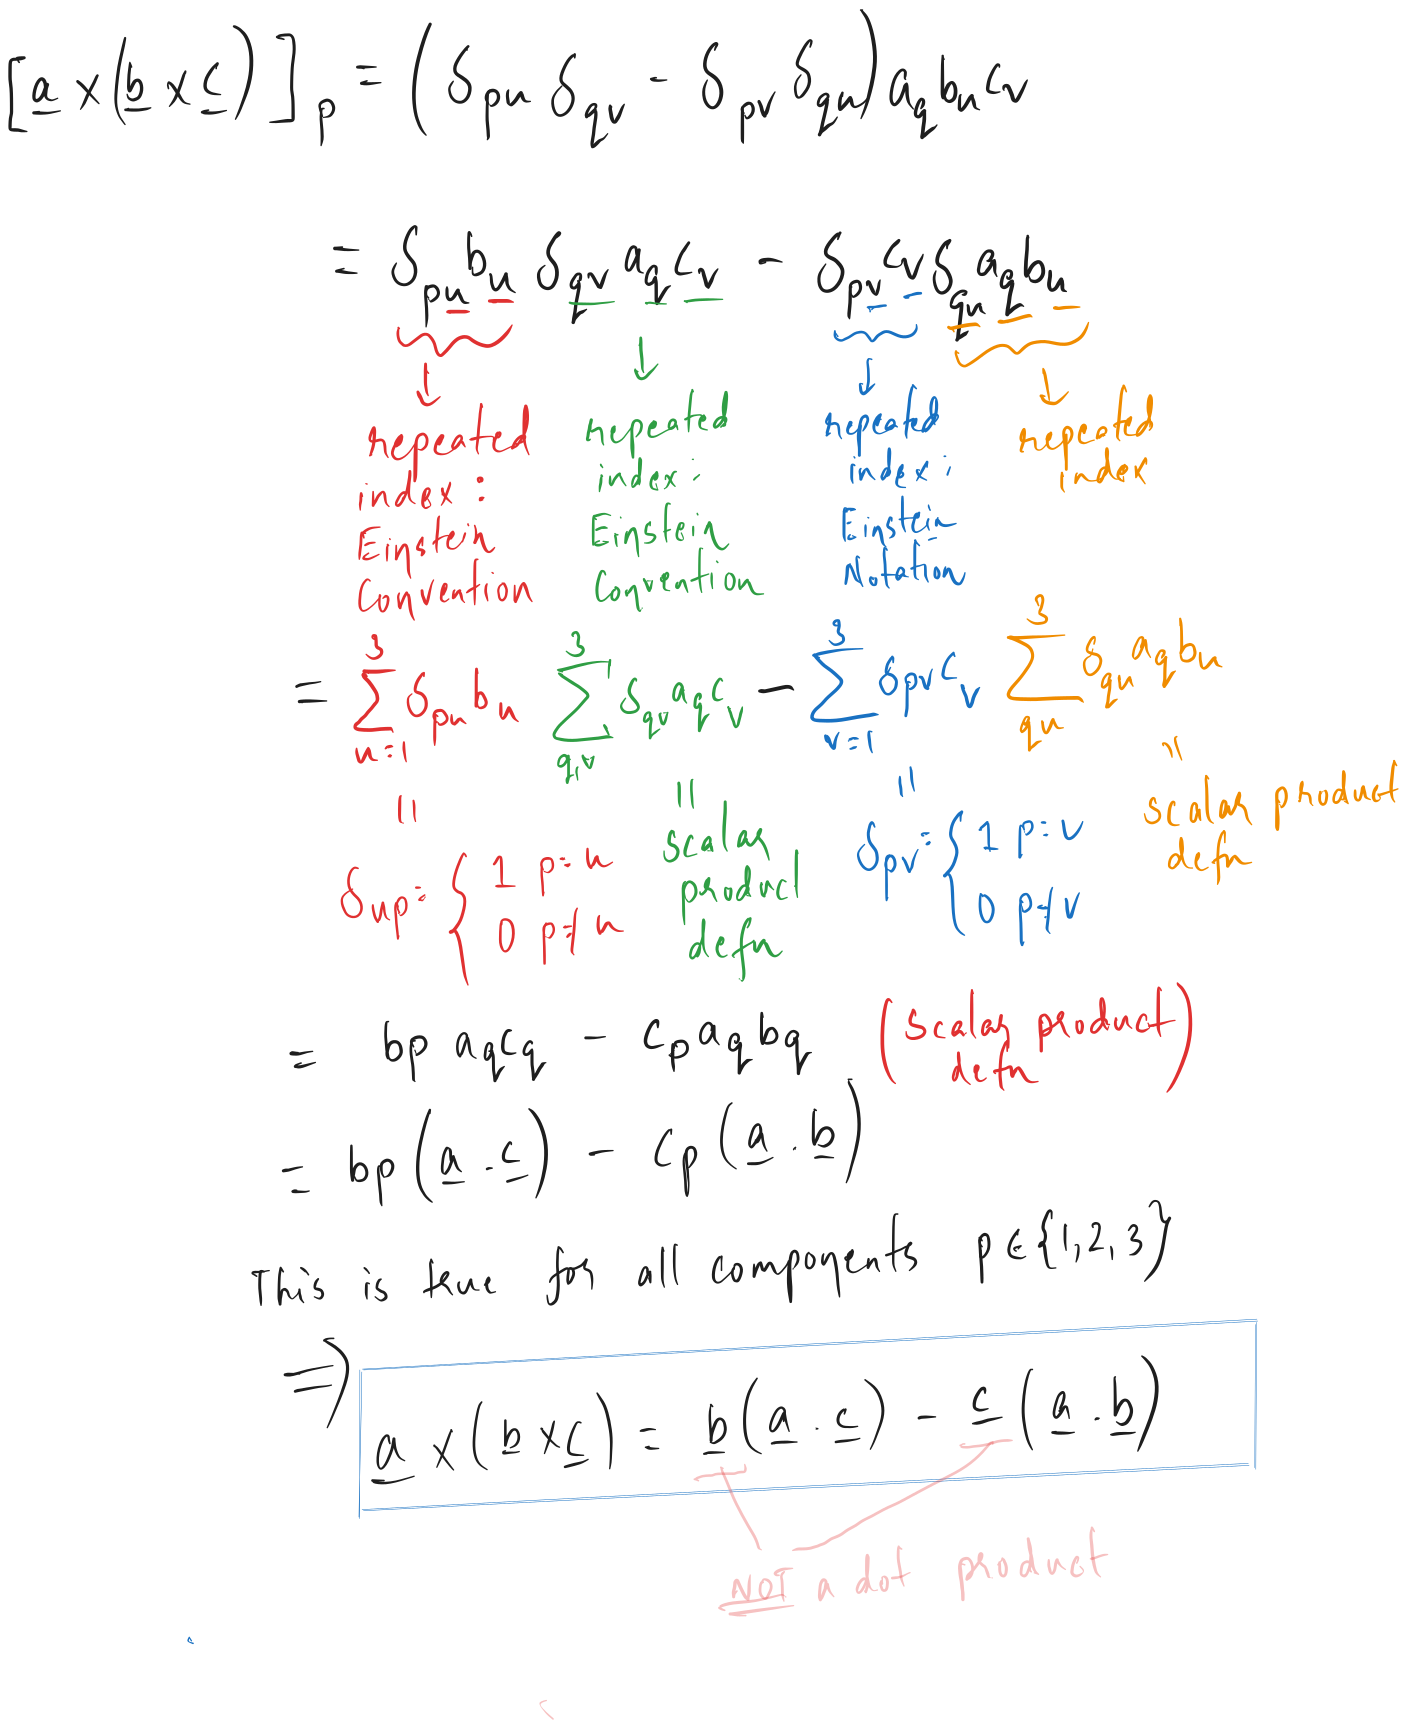
\includegraphics[scale=0.35]{triple-vector-product-proof.png}
	\caption{Triple Vector Product Proof}
	\label{fig:figure-triple-vector-product-proof}
\end{figure}

\clearpage

% \section{Vector Equation of Lines}

\begin{definition}[Vector Equation of Lines]
	The {\bf position vector} of $\underline{x}$ of an arbitrary point P(x,y,z) on the line in terms of $\underline{p}$ and $\underline{v}$
	\begin{equation}
		\label{eq: vector-lines}
		\underline{x} = \underline{p} + t\underline{v} \ \ \ \ \text{for } t \in \mathbb{R}
	\end{equation}
\end{definition}

\begin{figure}[H]
	\centering
	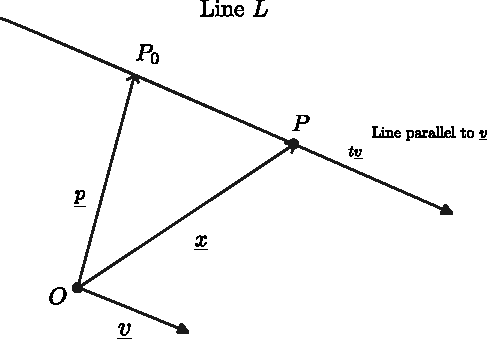
\includegraphics[scale=1.0]{vector-lines.pdf}
	\caption{Vector Line}
	\label{fig:figure-vector-lines}
\end{figure}

\subsection{Parametric Equation of a Line}
\begin{note}
	Every point $\underline{x}$ can be written as
	$$\underline{x} = x\hat{i} + y\hat{j} + z\hat{k}$$
	Therefore we can form a parametric equation of a line
\end{note}

\begin{definition}[Parametric Equation of a Line]
	\begin{equation}
		\label{eq: parametric-vector-lines}
		\begin{cases}
			x = x_0 + tv_1 \\
			y= y_0 + tv_2  \\
			z = z_0 + tv_3
		\end{cases}
		\ \ \ \ \ \text{for } t \in \mathbb{R}
	\end{equation}

\end{definition}

\subsection{Vector Equation of Line going through 2 points}
\begin{definition}
	Let $P$ and $Q$ be two points on the line and let their position vectors be $\underline{p}$ and $\underline{q}$ repectively. Then the
		{\bf direction vector} is:
	$$\vec{PQ} = \underline{q} - \underline{p}$$
	and the vector equation line is
	\begin{equation}
		\label{eq vector-lines-2p}
		\underline{x} = + t(\underline{q} - \underline{p}) \ \ \ \ \text{for } t \in \mathbb{R}
	\end{equation}
\end{definition}
The following diagram depicts this:

\begin{figure}[H]
	\centering
	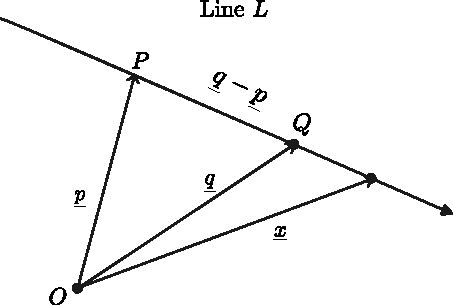
\includegraphics[scale=1.0]{vector-lines-2p.pdf}
	\caption{Vector Line}
	\label{fig:figure-vector-lines-2p}
\end{figure}

% \section{Vector Equation of Planes}
\begin{definition}[Vector Equation of Planes]
	Given a point $P$ with {\bf position vector} $\underline{p}$ and 2 vectors {\bf not} lying on the same line i.e. {\bf not collinear}, then there is a plane that passes
	through $P$ parallel to both $\underline{u}$ and $\underline{v}$

	The position vector of an {\em arbitrary} point $x$ is
	\begin{equation}
		\label{eq: vector-planes}
		\underline{x} = \underline{p} + s\underline{u} + t \underline{v} \ \ \ \ \text{for } s,t \in \mathbb{R}
	\end{equation}
\end{definition}
This is known as the {\bf plane spanned} by $\underline{u}$ and $\underline{v}$ going through $P$

\subsection{Parametric Equation of a line}
\begin{definition}
	\begin{equation}
		\label{eq: vector-planes-parametric}
		\begin{cases}
			x = x_0 + su_1 + tv_1 \\
			y = y_0 + su_2 + tv_2 \\
			z = z_0 + su_3 + tv_3
		\end{cases}
		\ \ \ \text{for } s,t \in \mathbb{R}
	\end{equation}
\end{definition}

\subsection{Vector Equation of Planes using 3 Points}
\begin{definition}
	Given 3 non-linear points $P, Q$ and $R$ with {\bf position vectors} $\underline{p}, \underline{q}$ and $\underline{r}$ respectively.
	Note that the vectors
	$$(\underline{p} - \underline{r}) \ \ \text{and} \ \  (\underline{q} - \underline{r})$$
	are two {\bf direction vectors parallel to the plane}. Then taking $r$ as the {\em starting point}, the equation of the plane becomes
	\begin{equation}
		\label{eq: vector-planes-3p}
		\underline{x} = \underline{r} + s(\underline{p} - \underline{r}) + t (\underline{q} - \underline{r}) \ \ \ \ \text{for } s,t \in \mathbb{R}
	\end{equation}
\end{definition}

\subsection{Normal Vector to a Plane}
Another way to define a plane is by noticing that (in 3d) there is exactly one line which is perpendicular to the plane. A vector parallel to this line is called a {\bf normal vector}.

\begin{note}[Unit Normal]
	If the {\bf normal vector} has unit length, then it called a {\bf \em unit normal} \\
	Thus if $\hat{n}$ is a unit normal to a plane then there is {\bf exactly one other} unit normal to the plane namely $-\hat{n}$
\end{note}

\begin{definition}[Equation of Plane using Normal Vector]
	If $\underline{p}$ is a {\bf position vector} of a {\em known} point in the plane and $\underline{x}$ is any {\bf arbitary point on the plane}, then
	$$( \underline{x} - \underline{p} ) $$
	is parallel to the plane and thus {\bf orthogonal} to the normal. Therefore equation of a plane can be given as
	\begin{equation}
		\label{eq: normal-vector-plane-eq}
		(\underline{x} - \underline{p})\cdot\underline{n} = 0 \ \ \ \ \ \ \ \ \ \ \ \ \ \  \text{(scalar product)}
	\end{equation}
	or multipying out the {\bf Scalar Product}
	$$\underline{x} \cdot \underline{n} = \underline{p} \cdot \underline{n}$$
\end{definition}

% \section{Change of Axes}

\subsection{Change of Origin}
Consider the following diagrams:
\begin{mycenter}
	\tikzset{every picture/.style={line width=0.75pt}} %set default line width to 0.75pt        

	\begin{tikzpicture}[x=0.75pt,y=0.75pt,yscale=-1,xscale=1]
		%uncomment if require: \path (0,402); %set diagram left start at 0, and has height of 402

		%Straight Lines [id:da4437652617379132] 
		\draw [color={rgb, 255:red, 208; green, 2; blue, 27 }  ,draw opacity=1 ]   (163.8,233.14) -- (153.42,92.92) ;
		\draw [shift={(153.27,90.92)}, rotate = 85.76] [color={rgb, 255:red, 208; green, 2; blue, 27 }  ,draw opacity=1 ][line width=0.75]    (10.93,-3.29) .. controls (6.95,-1.4) and (3.31,-0.3) .. (0,0) .. controls (3.31,0.3) and (6.95,1.4) .. (10.93,3.29)   ;
		%Straight Lines [id:da6919359366246228] 
		\draw [color={rgb, 255:red, 74; green, 144; blue, 226 }  ,draw opacity=1 ]   (337.38,204.91) -- (154.97,91.97) ;
		\draw [shift={(153.27,90.92)}, rotate = 31.76] [color={rgb, 255:red, 74; green, 144; blue, 226 }  ,draw opacity=1 ][line width=0.75]    (10.93,-3.29) .. controls (6.95,-1.4) and (3.31,-0.3) .. (0,0) .. controls (3.31,0.3) and (6.95,1.4) .. (10.93,3.29)   ;
		%Shape: Ellipse [id:dp7599712014506931] 
		\draw  [fill={rgb, 255:red, 0; green, 0; blue, 0 }  ,fill opacity=1 ] (161.56,231.4) .. controls (160.52,232.62) and (160.68,234.39) .. (161.92,235.36) .. controls (163.16,236.32) and (165,236.11) .. (166.04,234.89) .. controls (167.08,233.67) and (166.92,231.89) .. (165.68,230.93) .. controls (164.45,229.97) and (162.6,230.18) .. (161.56,231.4) -- cycle ;
		%Straight Lines [id:da7071864815591788] 
		\draw    (163.8,233.14) -- (335.4,205.23) ;
		\draw [shift={(337.38,204.91)}, rotate = 170.76] [color={rgb, 255:red, 0; green, 0; blue, 0 }  ][line width=0.75]    (10.93,-3.29) .. controls (6.95,-1.4) and (3.31,-0.3) .. (0,0) .. controls (3.31,0.3) and (6.95,1.4) .. (10.93,3.29)   ;
		%Shape: Ellipse [id:dp6834980772983773] 
		\draw  [fill={rgb, 255:red, 0; green, 0; blue, 0 }  ,fill opacity=1 ] (335.14,203.17) .. controls (334.1,204.39) and (334.26,206.16) .. (335.5,207.12) .. controls (336.73,208.09) and (338.58,207.88) .. (339.62,206.66) .. controls (340.65,205.43) and (340.5,203.66) .. (339.26,202.7) .. controls (338.02,201.74) and (336.18,201.95) .. (335.14,203.17) -- cycle ;
		%Shape: Ellipse [id:dp029391721000904147] 
		\draw  [fill={rgb, 255:red, 0; green, 0; blue, 0 }  ,fill opacity=1 ] (151.03,89.18) .. controls (149.99,90.4) and (150.15,92.17) .. (151.39,93.13) .. controls (152.62,94.1) and (154.47,93.89) .. (155.51,92.67) .. controls (156.55,91.44) and (156.39,89.67) .. (155.15,88.71) .. controls (153.92,87.75) and (152.07,87.96) .. (151.03,89.18) -- cycle ;

		% Text Node
		\draw (217.09,81.19) node [anchor=north west][inner sep=0.75pt]  [color={rgb, 255:red, 74; green, 144; blue, 226 }  ,opacity=1 ] [align=left] {$\displaystyle \underline{a}^{'}$};
		% Text Node
		\draw (151.96,239.31) node [anchor=north west][inner sep=0.75pt]   [align=left] {$\displaystyle O$};
		% Text Node
		\draw (349.48,196.33) node [anchor=north west][inner sep=0.75pt]   [align=left] {$\displaystyle O^{'}$};
		% Text Node
		\draw (237.69,224.04) node [anchor=north west][inner sep=0.75pt]   [align=left] {$\displaystyle \underline{s}$};
		% Text Node
		\draw (137,59) node [anchor=north west][inner sep=0.75pt]   [align=left] {$\displaystyle A$};
		% Text Node
		\draw (134,137) node [anchor=north west][inner sep=0.75pt]  [color={rgb, 255:red, 208; green, 2; blue, 27 }  ,opacity=1 ] [align=left] {$\displaystyle \underline{a}$};
	\end{tikzpicture}
\end{mycenter}
Here we have 2 vectors
\begin{itemize}
	\item $\displaystyle \overrightarrow{OO}$
	\item $\displaystyle \overrightarrow{O^{'}O}$
\end{itemize}

\begin{tcolorbox}[title=Shift of Origin]
	The {\bf shift} of origin is represented by $\underline{s}$ is {\em relative} to $O$, then
	$$\underline{u} = \underline{a} = \underline{s} + \underline{a^{'}} \Rightarrow \underline{a^{'}} = \underline{a} - \underline{s}$$
\end{tcolorbox}
\begin{note}
	\underline{s} {\bf could depend on time}
\end{note}

\begin{note}
	Consider the following diagram

	\begin{mycenter}
		\tikzset{every picture/.style={line width=0.75pt}} %set default line width to 0.75pt        

		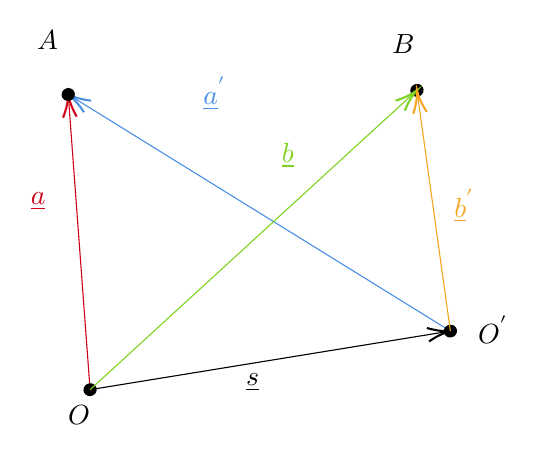
\begin{tikzpicture}[x=0.75pt,y=0.75pt,yscale=-1,xscale=1]
			%uncomment if require: \path (0,402); %set diagram left start at 0, and has height of 402

			%Straight Lines [id:da4437652617379132] 
			\draw [color={rgb, 255:red, 208; green, 2; blue, 27 }  ,draw opacity=1 ]   (163.8,233.14) -- (153.42,92.92) ;
			\draw [shift={(153.27,90.92)}, rotate = 85.76] [color={rgb, 255:red, 208; green, 2; blue, 27 }  ,draw opacity=1 ][line width=0.75]    (10.93,-3.29) .. controls (6.95,-1.4) and (3.31,-0.3) .. (0,0) .. controls (3.31,0.3) and (6.95,1.4) .. (10.93,3.29)   ;
			%Straight Lines [id:da6919359366246228] 
			\draw [color={rgb, 255:red, 74; green, 144; blue, 226 }  ,draw opacity=1 ]   (337.38,204.91) -- (154.97,91.97) ;
			\draw [shift={(153.27,90.92)}, rotate = 31.76] [color={rgb, 255:red, 74; green, 144; blue, 226 }  ,draw opacity=1 ][line width=0.75]    (10.93,-3.29) .. controls (6.95,-1.4) and (3.31,-0.3) .. (0,0) .. controls (3.31,0.3) and (6.95,1.4) .. (10.93,3.29)   ;
			%Shape: Ellipse [id:dp7599712014506931] 
			\draw  [fill={rgb, 255:red, 0; green, 0; blue, 0 }  ,fill opacity=1 ] (161.56,231.4) .. controls (160.52,232.62) and (160.68,234.39) .. (161.92,235.36) .. controls (163.16,236.32) and (165,236.11) .. (166.04,234.89) .. controls (167.08,233.67) and (166.92,231.89) .. (165.68,230.93) .. controls (164.45,229.97) and (162.6,230.18) .. (161.56,231.4) -- cycle ;
			%Straight Lines [id:da7071864815591788] 
			\draw    (163.8,233.14) -- (335.4,205.23) ;
			\draw [shift={(337.38,204.91)}, rotate = 170.76] [color={rgb, 255:red, 0; green, 0; blue, 0 }  ][line width=0.75]    (10.93,-3.29) .. controls (6.95,-1.4) and (3.31,-0.3) .. (0,0) .. controls (3.31,0.3) and (6.95,1.4) .. (10.93,3.29)   ;
			%Shape: Ellipse [id:dp6834980772983773] 
			\draw  [fill={rgb, 255:red, 0; green, 0; blue, 0 }  ,fill opacity=1 ] (335.14,203.17) .. controls (334.1,204.39) and (334.26,206.16) .. (335.5,207.12) .. controls (336.73,208.09) and (338.58,207.88) .. (339.62,206.66) .. controls (340.65,205.43) and (340.5,203.66) .. (339.26,202.7) .. controls (338.02,201.74) and (336.18,201.95) .. (335.14,203.17) -- cycle ;
			%Shape: Ellipse [id:dp029391721000904147] 
			\draw  [fill={rgb, 255:red, 0; green, 0; blue, 0 }  ,fill opacity=1 ] (151.03,89.18) .. controls (149.99,90.4) and (150.15,92.17) .. (151.39,93.13) .. controls (152.62,94.1) and (154.47,93.89) .. (155.51,92.67) .. controls (156.55,91.44) and (156.39,89.67) .. (155.15,88.71) .. controls (153.92,87.75) and (152.07,87.96) .. (151.03,89.18) -- cycle ;
			%Shape: Ellipse [id:dp487875436345539] 
			\draw  [fill={rgb, 255:red, 0; green, 0; blue, 0 }  ,fill opacity=1 ] (319.03,87.18) .. controls (317.99,88.4) and (318.15,90.17) .. (319.39,91.13) .. controls (320.62,92.1) and (322.47,91.89) .. (323.51,90.67) .. controls (324.55,89.44) and (324.39,87.67) .. (323.15,86.71) .. controls (321.92,85.75) and (320.07,85.96) .. (319.03,87.18) -- cycle ;
			%Straight Lines [id:da2129903038772052] 
			\draw [color={rgb, 255:red, 126; green, 211; blue, 33 }  ,draw opacity=1 ]   (163.8,233.14) -- (319.79,90.27) ;
			\draw [shift={(321.27,88.92)}, rotate = 137.51] [color={rgb, 255:red, 126; green, 211; blue, 33 }  ,draw opacity=1 ][line width=0.75]    (10.93,-3.29) .. controls (6.95,-1.4) and (3.31,-0.3) .. (0,0) .. controls (3.31,0.3) and (6.95,1.4) .. (10.93,3.29)   ;
			%Straight Lines [id:da6831431930714746] 
			\draw [color={rgb, 255:red, 245; green, 166; blue, 35 }  ,draw opacity=1 ]   (337.38,204.91) -- (321.54,90.9) ;
			\draw [shift={(321.27,88.92)}, rotate = 82.09] [color={rgb, 255:red, 245; green, 166; blue, 35 }  ,draw opacity=1 ][line width=0.75]    (10.93,-3.29) .. controls (6.95,-1.4) and (3.31,-0.3) .. (0,0) .. controls (3.31,0.3) and (6.95,1.4) .. (10.93,3.29)   ;

			% Text Node
			\draw (217.09,81.19) node [anchor=north west][inner sep=0.75pt]  [color={rgb, 255:red, 74; green, 144; blue, 226 }  ,opacity=1 ] [align=left] {$\displaystyle \underline{a}^{'}$};
			% Text Node
			\draw (151.96,239.31) node [anchor=north west][inner sep=0.75pt]   [align=left] {$\displaystyle O$};
			% Text Node
			\draw (349.48,196.33) node [anchor=north west][inner sep=0.75pt]   [align=left] {$\displaystyle O^{'}$};
			% Text Node
			\draw (237.69,224.04) node [anchor=north west][inner sep=0.75pt]   [align=left] {$\displaystyle \underline{s}$};
			% Text Node
			\draw (137,59) node [anchor=north west][inner sep=0.75pt]   [align=left] {$\displaystyle A$};
			% Text Node
			\draw (308,61) node [anchor=north west][inner sep=0.75pt]   [align=left] {$\displaystyle B$};
			% Text Node
			\draw (134,137) node [anchor=north west][inner sep=0.75pt]  [color={rgb, 255:red, 208; green, 2; blue, 27 }  ,opacity=1 ] [align=left] {$\displaystyle \underline{a}$};
			% Text Node
			\draw (255,113) node [anchor=north west][inner sep=0.75pt]  [color={rgb, 255:red, 126; green, 211; blue, 33 }  ,opacity=1 ] [align=left] {$\displaystyle \underline{b}$};
			% Text Node
			\draw (338,135) node [anchor=north west][inner sep=0.75pt]  [color={rgb, 255:red, 245; green, 166; blue, 35 }  ,opacity=1 ] [align=left] {$\displaystyle \underline{b}^{'}$};

		\end{tikzpicture}
	\end{mycenter}
	Let $\underline{a}$ and $\underline{b}$ represent  vectors  to $A$ and $B$ relative to $O$. Similarly let $\underline{a^{'}}$ and $\underline{b^{'}}$ represent vectors relative to $O^{\ '}$ .  Then:

	$$\underline{a}^{'}  \ - \ \underline{b}^{'}  = (\underline{a} - \underline{s})\  - \ (\underline{b}-\underline{s})  = \underline{a} - \underline{b}$$

	As we can see the {\bf displacement} from $\underline{a}$  to $\underline{b}$ is the {\bf same} as the {\bf displacement} from $\underline{a}^{'}$ to $\underline{b}^{'}$.
\end{note}


\subsection{Shifting and Changing Unit Vectors}


\lesson{1}{2023-10-23 16:36}{Newtownian Dynamics}
\chapter{Newtownian Dynamics}

In this section, we deal with {\bf particles} Particles are an idealization since real objects even if very small have very small a spatial extent.

	{\bf Particles} will be represented by a {\bf point in space} that movies in a trajectory denoted by $\underline{r}(t)$ which is a vector denoting its position at a time $t$ {\em relative} to a specified {\bf origin}.

\section{Basic Kinematics}
\subsection{Position of a particle}
\begin{definition}
	A point {\bf particle's} {\bf positon} at time $t$ on a {\bf trajectory} relative to an {\bf origin} $O$ can be described by a {\bf position vector}
		{\em relative} to an origin $O$

	The {\bf position vector} is $\underline{r}$ and can be represented using {\bf basis vectors}.
	\begin{equation}
		\label{eq: position-vector-particle}
		\underline{r}(t) = x\underline{i} + y\underline{j} + z\underline{k}
	\end{equation}

\end{definition}
\vspace{-10px}
\begin{mycenter}
	\tikzset{every picture/.style={line width=0.75pt}} %set default line width to 0.75pt        

	\begin{tikzpicture}[x=0.75pt,y=0.75pt,yscale=-1,xscale=1]
		%uncomment if require: \path (0,402); %set diagram left start at 0, and has height of 402

		%Curve Lines [id:da7249822784379534] 
		\draw    (108.1,195.3) .. controls (184.1,20.3) and (248.1,240.3) .. (367.1,64.3) ;
		%Straight Lines [id:da07486429812279405] 
		\draw    (203.5,258.3) -- (244.75,137.59) ;
		\draw [shift={(245.4,135.7)}, rotate = 108.87] [color={rgb, 255:red, 0; green, 0; blue, 0 }  ][line width=0.75]    (10.93,-3.29) .. controls (6.95,-1.4) and (3.31,-0.3) .. (0,0) .. controls (3.31,0.3) and (6.95,1.4) .. (10.93,3.29)   ;
		%Shape: Circle [id:dp6919219182514531] 
		\draw  [fill={rgb, 255:red, 0; green, 0; blue, 0 }  ,fill opacity=1 ] (242,135.7) .. controls (242,133.82) and (243.52,132.3) .. (245.4,132.3) .. controls (247.28,132.3) and (248.8,133.82) .. (248.8,135.7) .. controls (248.8,137.58) and (247.28,139.1) .. (245.4,139.1) .. controls (243.52,139.1) and (242,137.58) .. (242,135.7) -- cycle ;
		%Shape: Circle [id:dp2798104629473662] 
		\draw  [fill={rgb, 255:red, 0; green, 0; blue, 0 }  ,fill opacity=1 ] (200.1,258.3) .. controls (200.1,256.42) and (201.62,254.9) .. (203.5,254.9) .. controls (205.38,254.9) and (206.9,256.42) .. (206.9,258.3) .. controls (206.9,260.18) and (205.38,261.7) .. (203.5,261.7) .. controls (201.62,261.7) and (200.1,260.18) .. (200.1,258.3) -- cycle ;

		% Text Node
		\draw (213,245) node [anchor=north west][inner sep=0.75pt]   [align=left] {$\displaystyle O$};
		% Text Node
		\draw (241,108) node [anchor=north west][inner sep=0.75pt]   [align=left] {$\displaystyle P$};
		% Text Node
		\draw (236,173) node [anchor=north west][inner sep=0.75pt]   [align=left] {$\displaystyle \underline{r}( t)$};


	\end{tikzpicture}
\end{mycenter}

\begin{note}[Using Einstein Notation to describe position]

	Using {\bf Einstein's Notation} we can also represented it in the following way:
	$$\underline{r}(t) = \lambda_{a}\underline{e_{a}}$$

\end{note}

\subsection{Kinematics: Velocity and Acceleration}
In position vector of a particle (\ref{eq: position-vector-particle})  $\underline{r}$ assuming that the {\bf Orthonormal bais unit vectors} $\underline{i}, \underline{j}$ and $\underline{k}$ are {\bf constant}, we can write {\bf velocity} and {\bf acceleration} in the following way:

\clearpage

\subsubsection{Velocity}
Consider the following diagram:
\begin{mycenter}
	\tikzset{every picture/.style={line width=0.75pt}} %set default line width to 0.75pt        

	\begin{tikzpicture}[x=0.75pt,y=0.75pt,yscale=-1,xscale=1]
		%uncomment if require: \path (0,402); %set diagram left start at 0, and has height of 402

		%Curve Lines [id:da7249822784379534] 
		\draw    (108.1,195.3) .. controls (184.1,20.3) and (284.1,243.3) .. (403.1,67.3) ;
		%Straight Lines [id:da07486429812279405] 
		\draw    (203.5,258.3) -- (205.37,127.7) ;
		\draw [shift={(205.4,125.7)}, rotate = 90.82] [color={rgb, 255:red, 0; green, 0; blue, 0 }  ][line width=0.75]    (10.93,-3.29) .. controls (6.95,-1.4) and (3.31,-0.3) .. (0,0) .. controls (3.31,0.3) and (6.95,1.4) .. (10.93,3.29)   ;
		%Shape: Circle [id:dp6919219182514531] 
		\draw  [fill={rgb, 255:red, 0; green, 0; blue, 0 }  ,fill opacity=1 ] (202,125.7) .. controls (202,123.82) and (203.52,122.3) .. (205.4,122.3) .. controls (207.28,122.3) and (208.8,123.82) .. (208.8,125.7) .. controls (208.8,127.58) and (207.28,129.1) .. (205.4,129.1) .. controls (203.52,129.1) and (202,127.58) .. (202,125.7) -- cycle ;
		%Shape: Circle [id:dp2798104629473662] 
		\draw  [fill={rgb, 255:red, 0; green, 0; blue, 0 }  ,fill opacity=1 ] (200.1,258.3) .. controls (200.1,256.42) and (201.62,254.9) .. (203.5,254.9) .. controls (205.38,254.9) and (206.9,256.42) .. (206.9,258.3) .. controls (206.9,260.18) and (205.38,261.7) .. (203.5,261.7) .. controls (201.62,261.7) and (200.1,260.18) .. (200.1,258.3) -- cycle ;
		%Shape: Circle [id:dp4797202017377725] 
		\draw  [fill={rgb, 255:red, 0; green, 0; blue, 0 }  ,fill opacity=1 ] (244,132.7) .. controls (244,130.82) and (245.52,129.3) .. (247.4,129.3) .. controls (249.28,129.3) and (250.8,130.82) .. (250.8,132.7) .. controls (250.8,134.58) and (249.28,136.1) .. (247.4,136.1) .. controls (245.52,136.1) and (244,134.58) .. (244,132.7) -- cycle ;
		%Straight Lines [id:da797119100975235] 
		\draw [color={rgb, 255:red, 208; green, 2; blue, 27 }  ,draw opacity=1 ]   (203.5,258.3) -- (246.74,134.59) ;
		\draw [shift={(247.4,132.7)}, rotate = 109.27] [color={rgb, 255:red, 208; green, 2; blue, 27 }  ,draw opacity=1 ][line width=0.75]    (10.93,-3.29) .. controls (6.95,-1.4) and (3.31,-0.3) .. (0,0) .. controls (3.31,0.3) and (6.95,1.4) .. (10.93,3.29)   ;
		%Straight Lines [id:da3151106945356048] 
		\draw [color={rgb, 255:red, 126; green, 211; blue, 33 }  ,draw opacity=1 ]   (205.4,125.7) -- (245.43,132.37) ;
		\draw [shift={(247.4,132.7)}, rotate = 189.46] [color={rgb, 255:red, 126; green, 211; blue, 33 }  ,draw opacity=1 ][line width=0.75]    (10.93,-3.29) .. controls (6.95,-1.4) and (3.31,-0.3) .. (0,0) .. controls (3.31,0.3) and (6.95,1.4) .. (10.93,3.29)   ;

		% Text Node
		\draw (213,245) node [anchor=north west][inner sep=0.75pt]   [align=left] {$\displaystyle O$};
		% Text Node
		\draw (201,96) node [anchor=north west][inner sep=0.75pt]   [align=left] {$\displaystyle P$};
		% Text Node
		\draw (172,177) node [anchor=north west][inner sep=0.75pt]   [align=left] {$\displaystyle \underline{r}( t)$};
		% Text Node
		\draw (229,183) node [anchor=north west][inner sep=0.75pt]  [color={rgb, 255:red, 208; green, 2; blue, 27 }  ,opacity=1 ] [align=left] {$\displaystyle \underline{r}( t\ +\ \delta t)$};
		% Text Node
		\draw (221,105) node [anchor=north west][inner sep=0.75pt]  [color={rgb, 255:red, 126; green, 211; blue, 33 }  ,opacity=1 ] [align=left] {$\displaystyle \delta \underline{r}$};


	\end{tikzpicture}

\end{mycenter}
From the diagram above:
$$\delta\underline{r} = \underline{r}(t+\delta t) - \underline{r}(t) $$
Dividing by $\delta t$ and taking the {\bf limit} as $\delta \rightarrow 0$ we get
$$\dot{\underline{r}}(t) = \underline{v}(t) = \lim_{\delta t \to 0}\bigg(\frac{\underline{r}(t + \delta t) - \underline{r}(t)}{\delta t}\bigg)$$

\begin{definition}[Velocity of a Particle]
	\begin{equation}
		\label{eq: velocity-particle}
		\dot{\underline{r}} = \frac{d\underline{r}(t)}{dt}  = \lambda \dot{\underline{e_{a}}} = \dot{x}\underline{i} + \dot{y}\underline{j} +\dot{z}\underline{k}
	\end{equation}
\end{definition}

\subsubsection{acceleration}
Similarly {\bf acceleration} can be definined in the following way:
\begin{definition}[Velocity of a Particle]
	\begin{equation}
		\label{eq: acceleration-particle}
		\ddot{\underline{r}} = \frac{d\dot{\underline{r}}(t)}{dt}  = \lambda \ddot{\underline{e_{a}}} = \ddot{x}\underline{i} + \ddot{y}\underline{j} +\ddot{z}\underline{k}
	\end{equation}
\end{definition}

In terms of {\bf limits}
$$\ddot{\underline{r}}(t) = \dot{\underline{v}}(t) = \underline{a}(t) = \lim_{\delta t \to 0}\bigg(\frac{\underline{v}(t + \delta t) - \underline{v}(t)}{\delta t}\bigg)$$


\clearpage

\subsection{Examples of Trajectories}

\subsubsection{Straight Line Trajectory}
Consider the following diagram
\begin{mycenter}
	\tikzset{every picture/.style={line width=0.75pt}} %set default line width to 0.75pt        

	\begin{tikzpicture}[x=0.75pt,y=0.75pt,yscale=-1,xscale=1]
		%uncomment if require: \path (0,402); %set diagram left start at 0, and has height of 402

		%Straight Lines [id:da07486429812279405] 
		\draw    (203.5,258.3) -- (205.37,127.7) ;
		\draw [shift={(205.4,125.7)}, rotate = 90.82] [color={rgb, 255:red, 0; green, 0; blue, 0 }  ][line width=0.75]    (10.93,-3.29) .. controls (6.95,-1.4) and (3.31,-0.3) .. (0,0) .. controls (3.31,0.3) and (6.95,1.4) .. (10.93,3.29)   ;
		%Shape: Circle [id:dp6919219182514531] 
		\draw  [fill={rgb, 255:red, 0; green, 0; blue, 0 }  ,fill opacity=1 ] (202,125.7) .. controls (202,123.82) and (203.52,122.3) .. (205.4,122.3) .. controls (207.28,122.3) and (208.8,123.82) .. (208.8,125.7) .. controls (208.8,127.58) and (207.28,129.1) .. (205.4,129.1) .. controls (203.52,129.1) and (202,127.58) .. (202,125.7) -- cycle ;
		%Shape: Circle [id:dp2798104629473662] 
		\draw  [fill={rgb, 255:red, 0; green, 0; blue, 0 }  ,fill opacity=1 ] (200.1,258.3) .. controls (200.1,256.42) and (201.62,254.9) .. (203.5,254.9) .. controls (205.38,254.9) and (206.9,256.42) .. (206.9,258.3) .. controls (206.9,260.18) and (205.38,261.7) .. (203.5,261.7) .. controls (201.62,261.7) and (200.1,260.18) .. (200.1,258.3) -- cycle ;
		%Shape: Circle [id:dp4797202017377725] 
		\draw  [fill={rgb, 255:red, 0; green, 0; blue, 0 }  ,fill opacity=1 ] (264,100.7) .. controls (264,98.82) and (265.52,97.3) .. (267.4,97.3) .. controls (269.28,97.3) and (270.8,98.82) .. (270.8,100.7) .. controls (270.8,102.58) and (269.28,104.1) .. (267.4,104.1) .. controls (265.52,104.1) and (264,102.58) .. (264,100.7) -- cycle ;
		%Straight Lines [id:da797119100975235] 
		\draw [color={rgb, 255:red, 208; green, 2; blue, 27 }  ,draw opacity=1 ]   (203.5,258.3) -- (266.65,102.55) ;
		\draw [shift={(267.4,100.7)}, rotate = 112.07] [color={rgb, 255:red, 208; green, 2; blue, 27 }  ,draw opacity=1 ][line width=0.75]    (10.93,-3.29) .. controls (6.95,-1.4) and (3.31,-0.3) .. (0,0) .. controls (3.31,0.3) and (6.95,1.4) .. (10.93,3.29)   ;
		%Straight Lines [id:da8657231564938234] 
		\draw    (146,151.7) -- (371.1,57.3) ;
		%Shape: Right Angle [id:dp4402177451309871] 
		\draw  [color={rgb, 255:red, 245; green, 166; blue, 35 }  ,draw opacity=1 ] (295.76,82.07) -- (305.33,84.96) -- (302.44,94.53) ;

		% Text Node
		\draw (213,245) node [anchor=north west][inner sep=0.75pt]   [align=left] {$\displaystyle O$};
		% Text Node
		\draw (201,96) node [anchor=north west][inner sep=0.75pt]   [align=left] {$\displaystyle P$};
		% Text Node
		\draw (172,177) node [anchor=north west][inner sep=0.75pt]   [align=left] {$\displaystyle \underline{r_{0}}$};
		% Text Node
		\draw (229,183) node [anchor=north west][inner sep=0.75pt]  [color={rgb, 255:red, 208; green, 2; blue, 27 }  ,opacity=1 ] [align=left] {$\displaystyle \underline{r}( t)$};
		% Text Node
		\draw (288,55) node [anchor=north west][inner sep=0.75pt]  [color={rgb, 255:red, 245; green, 166; blue, 35 }  ,opacity=1 ] [align=left] {$\displaystyle \underline{v}( t)$};


	\end{tikzpicture}
\end{mycenter}

Using Vector equation of Lines (\ref{eq: vector-lines}), we get the following equation for $\underline{r}(t)$
$$\underline{r}(t) = \underline{r_{0}} + t\underline{v} \ \ \ \ \ \ \ \ \ \ \ \ \ \underline{v}, \underline{r_{0}}\ \ \ \text{are constants}$$
Then we can find the Velocity (\ref{eq: velocity-particle}) and Acceleration as (\ref{eq: acceleration-particle}) as
$$\begin{aligned}                          & \underline{v}(t) = \frac{d\underline{r}(t)}{dt} = \underline{\dot{r}}(t) = \underline{v}        \\ \\
                                         & \underline{a}(t) = \frac{d\underline{\dot{r}}(t)}{dt} = \ddot{\underline{r}(t)} = \underline{0}\end{aligned}$$

\subsubsection{Parabolic Trajectory}
\begin{definition}[Parabolic Trajectory]
	A parabolic trajectory is defined as
	\begin{equation}
		\label{eq: parabolic-trajectory}
		\underline{r} = \underline{r_{0}}+ \underline{v}_{0}t + \underline{a_{0}}\frac{1}{2}t^2
	\end{equation}
	where $\underline{v_0}$ and $\underline{r_0}$ are constants
\end{definition}
Acceleration (\ref{eq: acceleration-particle}) and Velocity (\ref{eq: velocity-particle}) are
\begin{itemize}
	\item $\displaystyle \underline{v}(t) = \frac{d\underline{r}(t)}{dt} = \underline{\dot{r}}(t) = \underline{v_{0}} + \underline{a_{0}}t$
	\item $\displaystyle \underline{a}(t) = \underline{\dot{v}}(t) = \frac{d}{dt}(\underline{v_{0}} + \underline{a_{0}}t) = \underline{a_0}$
\end{itemize}

{\bf Example of a Parabolic Trajectory:}
Consider the following equation:
$$\underline{r}(t) = (\underbrace{u_{0}\underline{i} + v_{0}\underline{k}}_{\underline{v_{0}}}) - \frac{1}{2}gt^{2}\underline{k}$$

\begin{mycenter}
	\tikzset{every picture/.style={line width=0.75pt}} %set default line width to 0.75pt        

	\begin{tikzpicture}[x=0.75pt,y=0.75pt,yscale=-1,xscale=1]
		%uncomment if require: \path (0,402); %set diagram left start at 0, and has height of 402

		%Straight Lines [id:da021686159454420983] 
		\draw    (150.1,91.3) -- (150.1,250.3) ;
		%Straight Lines [id:da9865222157984955] 
		\draw    (140,240) -- (328.1,240.3) ;
		%Shape: Right Angle [id:dp4412444494112757] 
		\draw   (143.39,98.71) -- (150.1,91.3) -- (157.33,97.84) ;
		%Shape: Right Angle [id:dp7802119319801154] 
		\draw   (321.88,232.47) -- (328.1,240.3) -- (320.46,246.37) ;
		%Curve Lines [id:da14645678527741524] 
		\draw    (150,240) .. controls (179.1,131.3) and (251.2,119.6) .. (289.1,240.3) ;
		%Straight Lines [id:da915058268090938] 
		\draw [color={rgb, 255:red, 208; green, 2; blue, 27 }  ,draw opacity=1 ]   (150,240) -- (252.42,173.39) ;
		\draw [shift={(254.1,172.3)}, rotate = 146.96] [color={rgb, 255:red, 208; green, 2; blue, 27 }  ,draw opacity=1 ][line width=0.75]    (10.93,-3.29) .. controls (6.95,-1.4) and (3.31,-0.3) .. (0,0) .. controls (3.31,0.3) and (6.95,1.4) .. (10.93,3.29)   ;

		% Text Node
		\draw (188,177) node [anchor=north west][inner sep=0.75pt]   [align=left] {$\displaystyle \underline{r}( t)$};
		% Text Node
		\draw (165,93) node [anchor=north west][inner sep=0.75pt]   [align=left] {$\displaystyle \underline{k}$};
		% Text Node
		\draw (144,65) node [anchor=north west][inner sep=0.75pt]   [align=left] {$\displaystyle z$};
		% Text Node
		\draw (281,245) node [anchor=north west][inner sep=0.75pt]   [align=left] {$\displaystyle \underline{i}$};
		% Text Node
		\draw (338,227) node [anchor=north west][inner sep=0.75pt]   [align=left] {$\displaystyle x$};


	\end{tikzpicture}
\end{mycenter}

Here, separating the {\bf components} if $\underline{i}$ and $\underline{k}$, we get the following ({\bf scalars}):
$$
	{x}(t) = u_{0}t \Rightarrow t = \frac{x(t)}{u_{0}}
$$
and substituting for in the value for $z(t)$ (component of $\underline{k}$),
$$\begin{aligned} z & = {v_{0}t} - \frac{1}{2}gt^{2 }                                           \\ \\
                  & = \frac{v_{0}\ x}{u_{0}} - \frac{1}{2}g\Big(\frac{x}{u_{0}}\Big)^{2 }     \\ \\
                  & = \frac{v_{0} \ x}{u_{0}}\Big(1 - \frac{1}{2}\frac{gx}{u_{0}\ v_{0}}\Big)\end{aligned}$$
And therefore as we can see, the equation for $z(t)$ is in the form of a {\bf parabola}.

\subsubsection{Circular Trajectory}
\begin{definition}[Circular Trajectory]
	Consider a particle {\bf trajectory} by the described by the following equations
	\begin{equation}
		\label{eq: circular-trajectory}
		\underline{r}(t) = a(\cos(\omega t)\underline{i} + \sin(\omega t)\underline{j})
	\end{equation}
\end{definition}

\begin{itemize}
	\item $x(t) = a\cos(\omega t)$ i.e. the $x$-component
	\item $y(t) = a\sin(\omega t)$ i.e. the $y$-component
\end{itemize}

\begin{note}
	$$x^{2}+ y^{2} = a^{2}\cos^{2}(\omega t) + a^{2}\cos^{2}(\omega t) \ \ \ \Rightarrow \ \ \  x^{2} + y^{2} = a^{2}$$
	which is the {\bf equation of a circle} of radius $a$.

\end{note}

{\bf Velocity in a circular trajectory}

First calculating the Velocity (\ref{eq: velocity-particle}),
$$\underline{\dot{r}}(t) = a(-\omega \sin(\omega t)\underline{i} + \omega\cos(\omega t)\underline{j})$$
where:
\begin{itemize}
	\item $\dot{x}(t) = -a\ \omega\sin(\omega t)$ i.e. the velocity in $x$-direction
	\item $\dot{y}(t) = a\ \omega\cos(\omega t)$ i.e. the velocity in $y$-direction
\end{itemize}
The {\bf magnitude} of velocity is:
$$\begin{aligned} \mid \underline{\dot{r}} \mid^{2} & = x^{2} + y^{2}                                                         \\ \\
                                                  & = a^{2}\omega^{2}\sin^{2}(\omega t) + a^{2}\omega^{2}\cos^{2}(\omega t) \\ \\
                                                  & = a^{2} \omega^{2}                                                      \\
                \Rightarrow\mid\underline{\dot{r}}\mid =  \mid\underline{v}\mid =a\omega\end{aligned}$$
We can see that velocity has a {\bf constant magnitude}, but is clearly {\bf changing in direction}.
The particle is moving in the {\bf anti-clockwise} direction. (This can be verified by \emph{checking any random point}).

	{\bf Acceleration in a circular trajectory}
Calculating the Acceleration (\ref{eq: acceleration-particle}),

$$\begin{aligned} \underline{\ddot{r}}(t) & = -a\omega^{2}(\cos(\omega t)\underline{i} + \sin(\omega t)\underline{j}) \\ \\
                                        & = -\omega^{2}\underline{r}\end{aligned}$$
So as we can see from the equation $\underline{\ddot{r}}(t) = -\omega^{2}\underline{r}$, we can see that the acceleration points downwards, i.e. opposite to the direction of $\underline{r}$ i.e. position vector.


\begin{figure}[H]
\centering
\tikzset{every picture/.style={line width=0.75pt}} %set default line width to 0.75pt        
\begin{tikzpicture}[x=0.75pt,y=0.75pt,yscale=-1,xscale=1]
%uncomment if require: \path (0,402); %set diagram left start at 0, and has height of 402

%Straight Lines [id:da021686159454420983] 
\draw    (230.1,98.3) -- (231.1,344.3) ;
%Straight Lines [id:da9865222157984955] 
\draw    (84.55,221.15) -- (376.65,221.45) ;
%Shape: Right Angle [id:dp4412444494112757] 
\draw   (222.98,105.32) -- (230.1,98.3) -- (236.95,105.24) ;
%Shape: Right Angle [id:dp7802119319801154] 
\draw   (369.99,213.99) -- (376.65,221.45) -- (369.37,227.94) ;
%Shape: Circle [id:dp5189182370807889] 
\draw   (138.82,221.3) .. controls (138.82,170.61) and (179.91,129.53) .. (230.6,129.53) .. controls (281.29,129.53) and (322.37,170.61) .. (322.37,221.3) .. controls (322.37,271.99) and (281.29,313.07) .. (230.6,313.07) .. controls (179.91,313.07) and (138.82,271.99) .. (138.82,221.3) -- cycle ;
%Straight Lines [id:da030770231855278496] 
\draw [color={rgb, 255:red, 208; green, 2; blue, 27 }  ,draw opacity=1 ]   (230.6,129.53) -- (179.1,130.27) ;
\draw [shift={(177.1,130.3)}, rotate = 359.17] [color={rgb, 255:red, 208; green, 2; blue, 27 }  ,draw opacity=1 ][line width=0.75]    (10.93,-3.29) .. controls (6.95,-1.4) and (3.31,-0.3) .. (0,0) .. controls (3.31,0.3) and (6.95,1.4) .. (10.93,3.29)   ;
%Straight Lines [id:da00482572515300661] 
\draw [color={rgb, 255:red, 208; green, 2; blue, 27 }  ,draw opacity=1 ]   (289.1,151.3) -- (251.5,112.73) ;
\draw [shift={(250.1,111.3)}, rotate = 45.73] [color={rgb, 255:red, 208; green, 2; blue, 27 }  ,draw opacity=1 ][line width=0.75]    (10.93,-3.29) .. controls (6.95,-1.4) and (3.31,-0.3) .. (0,0) .. controls (3.31,0.3) and (6.95,1.4) .. (10.93,3.29)   ;
%Straight Lines [id:da678334264237589] 
\draw    (230.6,221.3) -- (287.82,152.83) ;
\draw [shift={(289.1,151.3)}, rotate = 129.89] [color={rgb, 255:red, 0; green, 0; blue, 0 }  ][line width=0.75]    (10.93,-3.29) .. controls (6.95,-1.4) and (3.31,-0.3) .. (0,0) .. controls (3.31,0.3) and (6.95,1.4) .. (10.93,3.29)   ;
%Straight Lines [id:da503332446941831] 
\draw [color={rgb, 255:red, 126; green, 211; blue, 33 }  ,draw opacity=1 ]   (310.1,128.3) -- (290.45,149.82) ;
\draw [shift={(289.1,151.3)}, rotate = 312.4] [color={rgb, 255:red, 126; green, 211; blue, 33 }  ,draw opacity=1 ][line width=0.75]    (10.93,-3.29) .. controls (6.95,-1.4) and (3.31,-0.3) .. (0,0) .. controls (3.31,0.3) and (6.95,1.4) .. (10.93,3.29)   ;

% Text Node
\draw (262,181) node [anchor=north west][inner sep=0.75pt]   [align=left] {$\displaystyle \underline{r}( t)$};
% Text Node
\draw (239,71) node [anchor=north west][inner sep=0.75pt]   [align=left] {$\displaystyle \underline{j}$};
% Text Node
\draw (206,54) node [anchor=north west][inner sep=0.75pt]   [align=left] {$\displaystyle y$};
% Text Node
\draw (346,223) node [anchor=north west][inner sep=0.75pt]   [align=left] {$\displaystyle \underline{i}$};
% Text Node
\draw (384,210) node [anchor=north west][inner sep=0.75pt]   [align=left] {$\displaystyle x$};
% Text Node
\draw (195,104) node [anchor=north west][inner sep=0.75pt]  [color={rgb, 255:red, 208; green, 2; blue, 27 }  ,opacity=1 ] [align=left] {$\displaystyle \underline{v}$};
% Text Node
\draw (277,112) node [anchor=north west][inner sep=0.75pt]  [color={rgb, 255:red, 208; green, 2; blue, 27 }  ,opacity=1 ] [align=left] {$\displaystyle \underline{v}$};
% Text Node
\draw (312,109) node [anchor=north west][inner sep=0.75pt]  [color={rgb, 255:red, 126; green, 211; blue, 33 }  ,opacity=1 ] [align=left] {$\displaystyle \underline{a}$};


\end{tikzpicture}
\caption{Circular Trajectory} \label{fig: circular-trajectory-diagram}
\end{figure}

\clearpage

\section{Motion in Polar Co-ordinates}
\subsection{The polar co-ordinate system}
For any \textbf{vector} $\underline{x}$ on the $xy-plane$, we can introduce 2 {\bf unit vectors}
$$\underline{e_{r}} \ \ ,  \ \ \underline{e_{\theta}}$$
\begin{itemize}
	\item  $\underline{e_{r}}$ is the unit vector in the {\bf radial direction}
	\item  $\underline{e_{\theta}}$ is the unit vector in the {\bf azimuthal direction}
\end{itemize}


\begin{mycenter}
	\tikzset{every picture/.style={line width=0.75pt}} %set default line width to 0.75pt        

	\begin{tikzpicture}[x=0.75pt,y=0.75pt,yscale=-1,xscale=1]
		%uncomment if require: \path (0,402); %set diagram left start at 0, and has height of 402

		%Straight Lines [id:da021686159454420983] 
		\draw    (351.43,1.3) -- (353.12,398.08) ;
		%Straight Lines [id:da9865222157984955] 
		\draw    (105.55,199.45) -- (598.99,199.93) ;
		%Shape: Right Angle [id:dp4412444494112757] 
		\draw   (339.4,12.63) -- (351.43,1.3) -- (363,12.5) ;
		%Shape: Right Angle [id:dp7802119319801154] 
		\draw   (587.75,187.9) -- (598.99,199.93) -- (586.7,210.41) ;
		%Shape: Ellipse [id:dp5189182370807889] 
		\draw  [dash pattern={on 0.84pt off 2.51pt}] (197.24,199.69) .. controls (197.24,117.94) and (266.65,51.66) .. (352.27,51.66) .. controls (437.9,51.66) and (507.31,117.94) .. (507.31,199.69) .. controls (507.31,281.45) and (437.9,347.72) .. (352.27,347.72) .. controls (266.65,347.72) and (197.24,281.45) .. (197.24,199.69) -- cycle ;
		%Straight Lines [id:da678334264237589] 
		\draw    (352.27,199.69) -- (466.49,99.4) ;
		\draw [shift={(467.99,98.08)}, rotate = 138.71] [color={rgb, 255:red, 0; green, 0; blue, 0 }  ][line width=0.75]    (10.93,-3.29) .. controls (6.95,-1.4) and (3.31,-0.3) .. (0,0) .. controls (3.31,0.3) and (6.95,1.4) .. (10.93,3.29)   ;
		%Shape: Ellipse [id:dp07755096578723952] 
		\draw  [fill={rgb, 255:red, 0; green, 0; blue, 0 }  ,fill opacity=1 ] (462.84,98.08) .. controls (462.84,95.36) and (465.14,93.16) .. (467.99,93.16) .. controls (470.83,93.16) and (473.14,95.36) .. (473.14,98.08) .. controls (473.14,100.79) and (470.83,103) .. (467.99,103) .. controls (465.14,103) and (462.84,100.79) .. (462.84,98.08) -- cycle ;
		%Straight Lines [id:da47746960657082327] 
		\draw [color={rgb, 255:red, 74; green, 144; blue, 226 }  ,draw opacity=1 ]   (467.99,98.08) -- (505.35,64.99) ;
		\draw [shift={(506.84,63.67)}, rotate = 138.47] [color={rgb, 255:red, 74; green, 144; blue, 226 }  ,draw opacity=1 ][line width=0.75]    (10.93,-3.29) .. controls (6.95,-1.4) and (3.31,-0.3) .. (0,0) .. controls (3.31,0.3) and (6.95,1.4) .. (10.93,3.29)   ;
		%Straight Lines [id:da6490221790082495] 
		\draw [color={rgb, 255:red, 74; green, 144; blue, 226 }  ,draw opacity=1 ]   (467.99,98.08) -- (432.3,65.21) ;
		\draw [shift={(430.82,63.86)}, rotate = 42.64] [color={rgb, 255:red, 74; green, 144; blue, 226 }  ,draw opacity=1 ][line width=0.75]    (10.93,-3.29) .. controls (6.95,-1.4) and (3.31,-0.3) .. (0,0) .. controls (3.31,0.3) and (6.95,1.4) .. (10.93,3.29)   ;
		%Straight Lines [id:da4708485533590365] 
		\draw [color={rgb, 255:red, 208; green, 2; blue, 27 }  ,draw opacity=1 ] [dash pattern={on 0.84pt off 2.51pt}]  (430.82,63.86) -- (430.82,97.73) ;
		%Straight Lines [id:da004192017604060294] 
		\draw [color={rgb, 255:red, 208; green, 2; blue, 27 }  ,draw opacity=1 ] [dash pattern={on 0.84pt off 2.51pt}]  (467.99,98.08) -- (430.82,97.73) ;
		%Straight Lines [id:da2288290067165305] 
		\draw [color={rgb, 255:red, 208; green, 2; blue, 27 }  ,draw opacity=1 ] [dash pattern={on 0.84pt off 2.51pt}]  (507.1,98.08) -- (506.84,63.67) ;
		%Straight Lines [id:da8720909795724745] 
		\draw [color={rgb, 255:red, 208; green, 2; blue, 27 }  ,draw opacity=1 ] [dash pattern={on 0.84pt off 2.51pt}]  (507.1,98.08) -- (467.99,98.08) ;
		%Curve Lines [id:da03516890978243714] 
		\draw    (378.1,177.08) .. controls (395.1,172.08) and (398.1,191.08) .. (393.1,200.08) ;
		%Straight Lines [id:da8974682091961091] 
		\draw  [dash pattern={on 4.5pt off 4.5pt}]  (467.99,98.08) -- (468.1,204.08) ;
		%Straight Lines [id:da9922721724934852] 
		\draw  [dash pattern={on 4.5pt off 4.5pt}]  (352.1,98.08) -- (467.99,98.08) ;
		%Curve Lines [id:da6694541782019319] 
		\draw    (481.1,86.78) .. controls (493.1,81.78) and (493.54,99.08) .. (487.54,98.08) ;

		% Text Node
		\draw (421.62,136.07) node [anchor=north west][inner sep=0.75pt]   [align=left] {$\displaystyle r$};
		% Text Node
		\draw (384,71) node [anchor=north west][inner sep=0.75pt]  [color={rgb, 255:red, 208; green, 2; blue, 27 }  ,opacity=1 ] [align=left] {$\displaystyle \cos \theta $};
		% Text Node
		\draw (487.54,98.08) node [anchor=north west][inner sep=0.75pt]  [color={rgb, 255:red, 208; green, 2; blue, 27 }  ,opacity=1 ] [align=left] {$\displaystyle \cos \theta $};
		% Text Node
		\draw (378.1,177.08) node [anchor=north west][inner sep=0.75pt]   [align=left] {$\displaystyle \theta $};
		% Text Node
		\draw (423,28) node [anchor=north west][inner sep=0.75pt]  [color={rgb, 255:red, 74; green, 144; blue, 226 }  ,opacity=1 ] [align=left] {$\displaystyle \underline{e_{\theta }}$};
		% Text Node
		\draw (514,39) node [anchor=north west][inner sep=0.75pt]  [color={rgb, 255:red, 74; green, 144; blue, 226 }  ,opacity=1 ] [align=left] {$\displaystyle \underline{e_{r}}$};
		% Text Node
		\draw (421,98) node [anchor=north west][inner sep=0.75pt]  [color={rgb, 255:red, 208; green, 2; blue, 27 }  ,opacity=1 ] [align=left] {$\displaystyle sin\theta $};
		% Text Node
		\draw (513,70) node [anchor=north west][inner sep=0.75pt]  [color={rgb, 255:red, 208; green, 2; blue, 27 }  ,opacity=1 ] [align=left] {$\displaystyle sin\theta $};
		% Text Node
		\draw (462,200) node [anchor=north west][inner sep=0.75pt]   [align=left] {$\displaystyle x$};
		% Text Node
		\draw (334,85) node [anchor=north west][inner sep=0.75pt]   [align=left] {$\displaystyle y$};


	\end{tikzpicture}
\end{mycenter}

\begin{definition}[Relation between Cartesian and Polar Co-ordinates]
	\begin{align*}
		x = r \cos \theta  \ \ \ y =  r \sin \theta
	\end{align*}
	Where $\mid \underline{r} \mid = r$
\end{definition}

\begin{note}
	Just like basis vectors $\hat{i}$ and $\hat{j}$ in Cartesian co-ordinates, $\underline{e_{r}}$ and $\underline{e_{\theta}}$ are orthogonal to each other.
\end{note}

\clearpage

\subsection{Polar Basis Vectors}
\begin{definition}[Polar Orthonormal Basis]
	{\bf Unit Vectors} $$\underline{e_r} \ \ \  \text{and} \ \ \ \underline{e_{\theta}}$$
	form the {\bf orthonormal basis} for  the {\bf The Polar Co-Ordinate System}.
\end{definition}

Furthermore, the unit vectors $\underline{e_r}$ and $\underline{e_{\theta}}$ can be represented using {\bf cartesian basis vectors} $\underline{i}$ and $\underline{j}$

\begin{mycenter}
	\tikzset{every picture/.style={line width=0.75pt}} %set default line width to 0.75pt        

	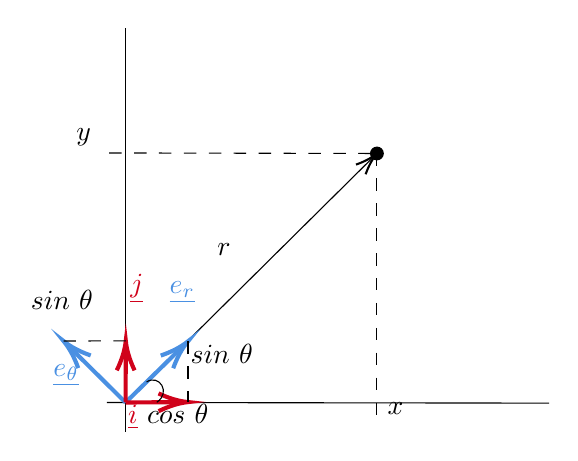
\begin{tikzpicture}[x=0.75pt,y=0.75pt,yscale=-1,xscale=1]
		%uncomment if require: \path (0,402); %set diagram left start at 0, and has height of 402

		%Straight Lines [id:da4134121928340384] 
		\draw    (270.1,119.68) -- (270.1,314.3) ;
		%Straight Lines [id:da5926046353448922] 
		\draw    (261,300) -- (474.1,300.3) ;
		%Straight Lines [id:da5096706615516877] 
		\draw    (270,300) -- (389.68,181.42) ;
		\draw [shift={(391.1,180.02)}, rotate = 135.27] [color={rgb, 255:red, 0; green, 0; blue, 0 }  ][line width=0.75]    (10.93,-3.29) .. controls (6.95,-1.4) and (3.31,-0.3) .. (0,0) .. controls (3.31,0.3) and (6.95,1.4) .. (10.93,3.29)   ;
		%Shape: Circle [id:dp7250045716603137] 
		\draw  [fill={rgb, 255:red, 0; green, 0; blue, 0 }  ,fill opacity=1 ] (388.05,180.02) .. controls (388.05,178.33) and (389.42,176.97) .. (391.1,176.97) .. controls (392.78,176.97) and (394.15,178.33) .. (394.15,180.02) .. controls (394.15,181.7) and (392.78,183.07) .. (391.1,183.07) .. controls (389.42,183.07) and (388.05,181.7) .. (388.05,180.02) -- cycle ;
		%Straight Lines [id:da348222394877604] 
		\draw  [dash pattern={on 4.5pt off 4.5pt}]  (391.1,180.02) -- (391.1,309.67) ;
		%Straight Lines [id:da6321585739703421] 
		\draw  [dash pattern={on 4.5pt off 4.5pt}]  (262.1,179.77) -- (391.1,180.02) ;
		%Straight Lines [id:da38254164085879216] 
		\draw [color={rgb, 255:red, 74; green, 144; blue, 226 }  ,draw opacity=1 ][line width=1.5]    (270,300) -- (297.96,272.6) ;
		\draw [shift={(300.1,270.5)}, rotate = 135.58] [color={rgb, 255:red, 74; green, 144; blue, 226 }  ,draw opacity=1 ][line width=1.5]    (14.21,-4.28) .. controls (9.04,-1.82) and (4.3,-0.39) .. (0,0) .. controls (4.3,0.39) and (9.04,1.82) .. (14.21,4.28)   ;
		%Straight Lines [id:da36292628024938856] 
		\draw [color={rgb, 255:red, 74; green, 144; blue, 226 }  ,draw opacity=1 ][line width=1.5]    (270,300) -- (242.23,272.49) ;
		\draw [shift={(240.1,270.38)}, rotate = 44.73] [color={rgb, 255:red, 74; green, 144; blue, 226 }  ,draw opacity=1 ][line width=1.5]    (14.21,-4.28) .. controls (9.04,-1.82) and (4.3,-0.39) .. (0,0) .. controls (4.3,0.39) and (9.04,1.82) .. (14.21,4.28)   ;
		%Straight Lines [id:da44840860590214315] 
		\draw [color={rgb, 255:red, 208; green, 2; blue, 27 }  ,draw opacity=1 ][line width=1.5]    (270,300) -- (270.09,273.3) ;
		\draw [shift={(270.1,270.3)}, rotate = 90.19] [color={rgb, 255:red, 208; green, 2; blue, 27 }  ,draw opacity=1 ][line width=1.5]    (14.21,-4.28) .. controls (9.04,-1.82) and (4.3,-0.39) .. (0,0) .. controls (4.3,0.39) and (9.04,1.82) .. (14.21,4.28)   ;
		%Straight Lines [id:da7989542731151809] 
		\draw [color={rgb, 255:red, 208; green, 2; blue, 27 }  ,draw opacity=1 ][line width=1.5]    (270,300) -- (297.1,299.82) ;
		\draw [shift={(300.1,299.8)}, rotate = 179.62] [color={rgb, 255:red, 208; green, 2; blue, 27 }  ,draw opacity=1 ][line width=1.5]    (14.21,-4.28) .. controls (9.04,-1.82) and (4.3,-0.39) .. (0,0) .. controls (4.3,0.39) and (9.04,1.82) .. (14.21,4.28)   ;
		%Straight Lines [id:da6303605300239684] 
		\draw  [dash pattern={on 4.5pt off 4.5pt}]  (300.1,270.5) -- (300.1,299.8) ;
		%Straight Lines [id:da1244707927752331] 
		\draw  [dash pattern={on 4.5pt off 4.5pt}]  (240.1,270.38) -- (270.1,270.3) ;
		%Curve Lines [id:da4414328655497084] 
		\draw    (280.1,290.13) .. controls (286.1,286.13) and (292.1,295.13) .. (285.05,299.9) ;

		% Text Node
		\draw (395,299) node [anchor=north west][inner sep=0.75pt]   [align=left] {$\displaystyle x$};
		% Text Node
		\draw (245,167) node [anchor=north west][inner sep=0.75pt]   [align=left] {$\displaystyle y$};
		% Text Node
		\draw (313,222) node [anchor=north west][inner sep=0.75pt]   [align=left] {$\displaystyle r$};
		% Text Node
		\draw (300.1,270.5) node [anchor=north west][inner sep=0.75pt]   [align=left] {$\displaystyle sin\ \theta $};
		% Text Node
		\draw (270,300) node [anchor=north west][inner sep=0.75pt]  [color={rgb, 255:red, 208; green, 2; blue, 27 }  ,opacity=1 ] [align=left] {$\displaystyle \underline{i}$};
		% Text Node
		\draw (271,237) node [anchor=north west][inner sep=0.75pt]  [color={rgb, 255:red, 208; green, 2; blue, 27 }  ,opacity=1 ] [align=left] {$\displaystyle \underline{j}$};
		% Text Node
		\draw (290,240.48) node [anchor=north west][inner sep=0.75pt]  [color={rgb, 255:red, 74; green, 144; blue, 226 }  ,opacity=1 ] [align=left] {$\displaystyle \underline{e_{r}}$};
		% Text Node
		\draw (234,280.48) node [anchor=north west][inner sep=0.75pt]  [color={rgb, 255:red, 74; green, 144; blue, 226 }  ,opacity=1 ] [align=left] {$\displaystyle \underline{e_{\theta }}$};
		% Text Node
		\draw (223.1,244.5) node [anchor=north west][inner sep=0.75pt]   [align=left] {$\displaystyle sin\ \theta $};
		% Text Node
		\draw (279.1,299.5) node [anchor=north west][inner sep=0.75pt]   [align=left] {$\displaystyle cos\ \theta $};


	\end{tikzpicture}
\end{mycenter}

As we can see from the diagram:
$$\underline{e_{r}}= \underline{i}\cos\theta + \underline{j}\sin\theta$$
and
$$\underline{e_{\theta}} = \pm \sin\theta \ \underline{i} + \mp \cos\theta\ \underline{j}$$
because $\underline{e_{r}}$ is {\bf orthogonal} to $\underline{e_{\theta}}$. Use the case from the diagram:
$$\underline{e_{\theta}} = \underline{i}\sin\theta - \underline{j}\cos\theta$$

\begin{definition}[Polar Basis Using Cartesian]
	\begin{flalign*}
		\underline{e_{r}}= \underline{i}\cos\theta + \underline{j}\sin\theta \\
		\underline{e_{\theta}} = \underline{i}\sin\theta - \underline{j}\cos\theta
	\end{flalign*}
\end{definition}

\subsubsection{Properties of Polar Orthonormal Basis}
\begin{theorem}
	Since $\underline{e_r}$ and $\underline{e_\theta}$ are \textbf{orthogonal},
	$$\underline{e_r} \cdot \underline{e_\theta} = 0$$
	(scalar product is 0)
\end{theorem}

\clearpage

\begin{theorem}
	The cross product (\ref{eq:cross-product-formula})
	$$\underline{e_r} \times \underline{e_{\theta}} = 0$$
\end{theorem}
\begin{proof}
	$$\begin{aligned} \underline{e_{r}} \times \underline{e_{\theta}} & = (\underline{i}\cos\theta + \underline{j}\sin\theta) \times ( \underline{i}\sin\theta - \underline{j}\cos\theta) \\ \\ &= (\cos^{2}\theta+ \sin^{2}\theta)\underline{i} \times \underline{j} \\ \\
                                                                & = \underline{k}                                                                                                   \\ \\\end{aligned}$$
\end{proof}

\subsection{Derivatives of Polar Orthonormal Basis Vectors}
We assume that the {\bf angle changes with time}, i.e.
$$\theta = \theta\left( t \right) $$
and therefore the {\bf polar basis vectors} are {\bf NOT CONSTANT}.

\subsubsection{First Derivative}
First we will compute the first derivatives $\underline{\dot{e_{r}}}$ and $\underline{\dot{e_{\theta}}}$.
\begin{enumerate}
	\item Computing $\underline{\dot{e_r}}$
	      $$\begin{aligned} \underline{\dot{e_{r}}} & = \frac{d}{dt}\Big(\underline{i}\cos\theta  + \underline{j}\sin\theta\Big)         \\ \\
                                        & = - \dot{\theta}\sin(\theta) \underline{i} + \dot{\theta}\cos(\theta)\underline{j} \\ \\
                                        & = \dot{\theta}(-\sin(\theta)\underline{i} + \cos(\theta)\underline{j})             \\ \\
                                        & = \dot{\theta}\ \underline{e_{\theta}}\end{aligned}$$
	      \begin{definition}[First derivative of $\underline{e_r}$]
		      $$\begin{aligned} \underline{\dot{e_{r}}} &= \dot{\theta}\ \underline{e_{\theta}}\\ \\ &= - \dot{\theta}\sin(\theta) \underline{i} + \dot{\theta}\cos(\theta)\underline{j} \end{aligned}$$
	      \end{definition}

	      \clearpage
	\item Computing $\underline{\dot{e_{\theta}}}$
	      $$\begin{aligned} \underline{\dot{e_{r}}} & = \frac{d}{dt}\Big(-\sin(\theta)\underline{i}  + \cos(\theta)\underline{j}\Big)    \\ \\
                                        & = - \dot{\theta}\cos(\theta) \underline{i} - \dot{\theta}\sin(\theta)\underline{j} \\ \\
                                        & = -\dot{\theta}(\cos(\theta)\underline{i} + \sin(\theta)\underline{j})             \\ \\
                                        & = \dot{\theta}\ \underline{e_{r}}\end{aligned}$$

	      \begin{definition}[First derivative of $\underline{e_r}$]
		      $$\begin{aligned} \underline{\dot{e_{\theta}}} &= -\dot{\theta}\ \underline{e_{r}}\\ \\ &= - \dot{\theta}\cos(\theta) \underline{i} - \dot{\theta}\sin(\theta)\underline{j} \end{aligned}$$
	      \end{definition}
\end{enumerate}

\subsection{Position Vector in Polar Co-ordinates}

\begin{definition}
	In polar co-ordinates, {\bf the position vector} i.e. the position of a particle is simply
	$$\underline{r} = r\ \underline{e_{r}}$$
\end{definition}
\vspace{4px}
\begin{mycenter}
	\tikzset{every picture/.style={line width=0.75pt}} %set default line width to 0.75pt        

	\begin{tikzpicture}[x=0.75pt,y=0.75pt,yscale=-1,xscale=1]
		%uncomment if require: \path (0,402); %set diagram left start at 0, and has height of 402

		%Straight Lines [id:da4134121928340384] 
		\draw    (251.1,37.68) -- (251.1,232.3) ;
		%Straight Lines [id:da5926046353448922] 
		\draw    (242,218) -- (455.1,218.3) ;
		%Straight Lines [id:da5096706615516877] 
		\draw    (251,218) -- (370.68,99.42) ;
		\draw [shift={(372.1,98.02)}, rotate = 135.27] [color={rgb, 255:red, 0; green, 0; blue, 0 }  ][line width=0.75]    (10.93,-3.29) .. controls (6.95,-1.4) and (3.31,-0.3) .. (0,0) .. controls (3.31,0.3) and (6.95,1.4) .. (10.93,3.29)   ;
		%Shape: Circle [id:dp7250045716603137] 
		\draw  [fill={rgb, 255:red, 0; green, 0; blue, 0 }  ,fill opacity=1 ] (369.05,98.02) .. controls (369.05,96.33) and (370.42,94.97) .. (372.1,94.97) .. controls (373.78,94.97) and (375.15,96.33) .. (375.15,98.02) .. controls (375.15,99.7) and (373.78,101.07) .. (372.1,101.07) .. controls (370.42,101.07) and (369.05,99.7) .. (369.05,98.02) -- cycle ;
		%Straight Lines [id:da38254164085879216] 
		\draw [color={rgb, 255:red, 74; green, 144; blue, 226 }  ,draw opacity=1 ][line width=1.5]    (251,218) -- (278.96,190.6) ;
		\draw [shift={(281.1,188.5)}, rotate = 135.58] [color={rgb, 255:red, 74; green, 144; blue, 226 }  ,draw opacity=1 ][line width=1.5]    (14.21,-4.28) .. controls (9.04,-1.82) and (4.3,-0.39) .. (0,0) .. controls (4.3,0.39) and (9.04,1.82) .. (14.21,4.28)   ;
		%Straight Lines [id:da36292628024938856] 
		\draw [color={rgb, 255:red, 74; green, 144; blue, 226 }  ,draw opacity=1 ][line width=1.5]    (251,218) -- (223.23,190.49) ;
		\draw [shift={(221.1,188.38)}, rotate = 44.73] [color={rgb, 255:red, 74; green, 144; blue, 226 }  ,draw opacity=1 ][line width=1.5]    (14.21,-4.28) .. controls (9.04,-1.82) and (4.3,-0.39) .. (0,0) .. controls (4.3,0.39) and (9.04,1.82) .. (14.21,4.28)   ;
		%Curve Lines [id:da4414328655497084] 
		\draw    (266.05,203.25) .. controls (268.1,201.3) and (276.1,213.3) .. (269.1,218.3) ;
		%Shape: Right Angle [id:dp2584901282247881] 
		\draw   (240.54,48.53) -- (251.1,37.68) -- (261.61,47.91) ;
		%Shape: Right Angle [id:dp7209517007920886] 
		\draw   (444.39,207.61) -- (455.1,218.3) -- (444.74,228.68) ;
		%Shape: Arc [id:dp1759431846665106] 
		\draw  [draw opacity=0][dash pattern={on 0.84pt off 2.51pt}] (245.77,62.86) .. controls (253.2,61.83) and (260.79,61.3) .. (268.5,61.3) .. controls (357.9,61.3) and (430.55,132.88) .. (432.08,221.77) -- (268.5,224.62) -- cycle ; \draw  [dash pattern={on 0.84pt off 2.51pt}] (245.77,62.86) .. controls (253.2,61.83) and (260.79,61.3) .. (268.5,61.3) .. controls (357.9,61.3) and (430.55,132.88) .. (432.08,221.77) ;

		% Text Node
		\draw (294,140) node [anchor=north west][inner sep=0.75pt]   [align=left] {$\displaystyle r$};
		% Text Node
		\draw (271,158.48) node [anchor=north west][inner sep=0.75pt]  [color={rgb, 255:red, 74; green, 144; blue, 226 }  ,opacity=1 ] [align=left] {$\displaystyle \underline{e_{r}}$};
		% Text Node
		\draw (215,198.48) node [anchor=north west][inner sep=0.75pt]  [color={rgb, 255:red, 74; green, 144; blue, 226 }  ,opacity=1 ] [align=left] {$\displaystyle \underline{e_{\theta }}$};
		% Text Node
		\draw (281,194) node [anchor=north west][inner sep=0.75pt]   [align=left] {$\displaystyle \theta $};


	\end{tikzpicture}
\end{mycenter}

\subsection{Polar Velocity and Acceleration}

\subsubsection{Velocity}
Computing {\bf velocity} in {\bf polar co-ordinates}:
$$\begin{aligned} \dot{\underline{r}} & = \frac{d}{dt}\Big(r \ \underline{e_{r}}\Big)                                                              \\ \\
                                    & = \dot{r}\ \underline{e_{r}} + r\ \dot{\theta}\ \underline{e_{\theta}} \ \ \ \ \ \ \ \ \text{product rule}\end{aligned}$$

\begin{definition}[Velocity in Polar co-ordinates]
	\begin{equation}
		\label{eq: velocity-polar}
		\underline{\dot{r}} = \dot{r}\ \underline{e_{r}} + r\ \dot{\theta}\ \underline{e_{\theta}}
	\end{equation}
\end{definition}

\subsubsection{Acceleration}
Computing {\bf Acceleration} in {\bf polar co-ordinates}:
$$\begin{aligned} \underline{\ddot{r}} & = \frac{d}{dt}\Big(\dot{r}(t)\Big)                                                                                                                                                              \\ \\
                                     & = \frac{d}{dt}\Big(\dot{r}\underline{e_{r}} + r\dot{\theta}\underline{e_{\theta}} \Big)                                                                                                         \\ \\
                                     & = \ddot{r}\underline{e_{r}}+ \dot{r}\dot{e_{r}}+ \dot{r}\dot{\theta}\underline{e_{\theta}} + r\ddot{\theta}\underline{e_{\theta}} + r\dot{\theta}\underline{\dot{e_{\theta}}}                   \\ \\
                                     & = \ddot{r}\underline{e_{r}} + \dot{r}\dot{\theta}\underline{e_{\theta}} + \dot{r}\dot{\theta}\underline{e_{\theta}} + r\ddot{\theta}\underline{e_{\theta}} - r\dot{\theta}^{2}\underline{e_{r}} \\ \\
                                     & = (\ddot{r} - r\dot{\theta}^{2})\underline{e_{r}} + (r\ddot{\theta} + 2\dot{r}\dot{\theta})\underline{e_{\theta}}\end{aligned}$$

\begin{definition}[Acceleration in Polar co-ordinates]
	\begin{equation}
		\label{eq: velocity-acceleration}
		\ddot{r} = (\ddot{r} - r\dot{\theta}^{2})\underline{e_{r}} + (r\ddot{\theta} + 2\dot{r}\dot{\theta})\underline{e_{\theta}}
	\end{equation}
\end{definition}

\subsection{Cross Product Between Position and Velocity in Polar}
We want to compute the cross product \ref{eq:cross-product-formula-2}
$$\underline{r} \times \underline{\dot{r}}$$
We can compute it as follows
$$\begin{aligned} \underline{r} \times \underline{\dot{r}} & = \underline{r} \times (\dot{r} \underline{e_{r}}+ r\dot{\theta}\underline{e_{\theta}})                                     \\ \\
                                                         & = (\underline{r} \times \dot{r}\underline{{e_{r}}}) + (\underline{r} \times r\dot{\theta}\underline{e_{\theta}})            \\ \\
                                                         & =  (r\underline{e_{r}} \times \dot{r}\underline{{e_{r}}}) + (r\underline{e_{}r} \times r\dot{\theta}\underline{e_{\theta}}) \\ \\
                                                         & =  r\dot{r}(\underline{e_{r}}\times \underline{e_{r}}) + r^{2}\dot{\theta}(\underline{e_{r}}+ \underline{e_{\theta}})       \\ \\
                                                         & = r^{2}\dot{\theta}\underline{k}\end{aligned}$$

\begin{note}
	We have used the {\bf properties of cross product} on {cartesian and polar basis vectors}

\end{note}

\begin{definition}[Cross Product b/w Position and Velocity in Polar]
	\begin{equation}
		\label{eq: plolar-cross-vel-pos}
		\underline{r} \times \underline{\dot{r}} =  r^{2}\dot{\theta}\underline{k}
	\end{equation}
\end{definition}

\begin{note}
	$\dot{r} \neq \mid \underline{\dot{r}} \mid$ or rather
	$$\dot{r} = \underline{\dot{r}} \cdot \underline{e_{r}} = \frac{\underline{r}\cdot\underline{\dot{r}}}{r} \ \ \ \ \ \text{while, } \mid\underline{r} \mid = \sqrt{\dot{r}^2+r^2\dot{\theta}^2}$$

\end{note}

\section{Inertial Frames}

The Laws of Physics are the {\bf SAME} in {\bf ALL} inertial frames. Inertial frames are frames of reference which are not accelerating and where Newton's law of inertia holds.

\subsection{Convertting between Inertial frames}
Consider the following diagram:

\begin{mycenter}

	\tikzset{every picture/.style={line width=0.75pt}} %set default line width to 0.75pt        

	\begin{tikzpicture}[x=0.75pt,y=0.75pt,yscale=-1,xscale=1]
		%uncomment if require: \path (0,402); %set diagram left start at 0, and has height of 402

		%Curve Lines [id:da6494685558841314] 
		\draw    (180.1,126.3) .. controls (224.1,15.3) and (279.1,180.3) .. (404.1,96.3) ;
		%Shape: Circle [id:dp014402697974219558] 
		\draw  [fill={rgb, 255:red, 0; green, 0; blue, 0 }  ,fill opacity=1 ] (306,118.55) .. controls (306,116.59) and (307.59,115) .. (309.55,115) .. controls (311.51,115) and (313.1,116.59) .. (313.1,118.55) .. controls (313.1,120.51) and (311.51,122.1) .. (309.55,122.1) .. controls (307.59,122.1) and (306,120.51) .. (306,118.55) -- cycle ;
		%Straight Lines [id:da09609682920605778] 
		\draw    (252.1,202.3) -- (308.42,120.2) ;
		\draw [shift={(309.55,118.55)}, rotate = 124.45] [color={rgb, 255:red, 0; green, 0; blue, 0 }  ][line width=0.75]    (10.93,-3.29) .. controls (6.95,-1.4) and (3.31,-0.3) .. (0,0) .. controls (3.31,0.3) and (6.95,1.4) .. (10.93,3.29)   ;
		%Shape: Circle [id:dp01339246524637483] 
		\draw  [fill={rgb, 255:red, 0; green, 0; blue, 0 }  ,fill opacity=1 ] (248.55,202.3) .. controls (248.55,200.34) and (250.14,198.75) .. (252.1,198.75) .. controls (254.06,198.75) and (255.65,200.34) .. (255.65,202.3) .. controls (255.65,204.26) and (254.06,205.85) .. (252.1,205.85) .. controls (250.14,205.85) and (248.55,204.26) .. (248.55,202.3) -- cycle ;
		%Straight Lines [id:da544230444191167] 
		\draw [color={rgb, 255:red, 74; green, 144; blue, 226 }  ,draw opacity=1 ]   (384.1,216.3) -- (310.76,120.14) ;
		\draw [shift={(309.55,118.55)}, rotate = 52.67] [color={rgb, 255:red, 74; green, 144; blue, 226 }  ,draw opacity=1 ][line width=0.75]    (10.93,-3.29) .. controls (6.95,-1.4) and (3.31,-0.3) .. (0,0) .. controls (3.31,0.3) and (6.95,1.4) .. (10.93,3.29)   ;
		%Shape: Circle [id:dp8571174104651734] 
		\draw  [fill={rgb, 255:red, 0; green, 0; blue, 0 }  ,fill opacity=1 ] (380.55,216.3) .. controls (380.55,214.34) and (382.14,212.75) .. (384.1,212.75) .. controls (386.06,212.75) and (387.65,214.34) .. (387.65,216.3) .. controls (387.65,218.26) and (386.06,219.85) .. (384.1,219.85) .. controls (382.14,219.85) and (380.55,218.26) .. (380.55,216.3) -- cycle ;
		%Straight Lines [id:da46992008958547604] 
		\draw [color={rgb, 255:red, 208; green, 2; blue, 27 }  ,draw opacity=1 ]   (252.1,202.3) -- (382.11,216.09) ;
		\draw [shift={(384.1,216.3)}, rotate = 186.05] [color={rgb, 255:red, 208; green, 2; blue, 27 }  ,draw opacity=1 ][line width=0.75]    (10.93,-3.29) .. controls (6.95,-1.4) and (3.31,-0.3) .. (0,0) .. controls (3.31,0.3) and (6.95,1.4) .. (10.93,3.29)   ;

		% Text Node
		\draw (227,200) node [anchor=north west][inner sep=0.75pt]   [align=left] {$\displaystyle O$};
		% Text Node
		\draw (384.1,212.75) node [anchor=north west][inner sep=0.75pt]   [align=left] {$\displaystyle O^{'}$};
		% Text Node
		\draw (243,144) node [anchor=north west][inner sep=0.75pt]   [align=left] {$\displaystyle r( t)$};
		% Text Node
		\draw (357,142) node [anchor=north west][inner sep=0.75pt]   [align=left] {$\displaystyle r^{'}$(t)};
		% Text Node
		\draw (301,217) node [anchor=north west][inner sep=0.75pt]   [align=left] {$\displaystyle s( t)$};


	\end{tikzpicture}

\end{mycenter}

Here
\begin{itemize}
	\item The vector $r(t)$ is the position vector of a particle in the inertial frame $O$/relative to $0$.
	\item The vector $r'(t)$ is the position vector of the same particle in the inertial frame $O'$/relative to $O'$.
	\item The vector $s(t)$ represents the shift between the two frames.
\end{itemize}

$$\begin{aligned}\underline{r}(t) = \underline{r^{'}}(t) + \underline{s}(t) & \Rightarrow \underline{\dot{r}}(t) = \underline{\dot{r}}^{'}(t) + \underline{\dot{s}}(t)    \\ \\
                                                                          & \Rightarrow \underline{\ddot{r}}(t) = \underline{\ddot{r}}^{'}(t) + \underline{\ddot{s}}(t)\end{aligned}$$

\clearpage
Since we are working with {\bf inertial frames}, they both must have {\bf constant relative velocity}
$$\underline{s}^{'} = \text{ constant } = \underline{s}^{''}\left(t  \right) = 0$$
i.e. the shift acceleration/relative acceleration is zero.

\begin{definition}[Inertial Frames]
	An {\bf inertial frame} is a frame of reference which is not accelerating and where Newton's law of inertia holds. \\
	If we an inertial frame, {\bf the relative/shift acceleration is 0}
	\begin{equation}
		s^{''}(t) = 0 \tag{$*$} \label{eq: gallilean}
	\end{equation}
	and therefore
	$$\ddot{r}(t) = \ddot{r}^{'}(t)$$

\end{definition}

\subsection{Gallilean Transformation}
We have seen from (\ref{eq: gallilean}) that to have an inertial frame we had
$$\underline{\ddot{s}}\left(t  \right) $$
And then we can solve this differential equation with respect to $t$ to get
$$\underline{\ddot{s}}\left(t  \right) = a + ut$$
where $u$ is a {\bf constant velocity} and $a$ is a {\bf shift in origin}. This is also known as {\bf Gallilean transformation}.

\begin{definition}[Gallilean Transformation]
	A Gallilean Transformation is when the the {\bf shift vector} $s(t)$ is the following:
	\begin{equation}
		\label{eq: gallilean-transformation}
		s(t) = a + ut
	\end{equation}
\end{definition}

\section{Newton's Laws of Motion}

\subsection{Inertia}
\begin{definition}[Law of Inertia]
	Any body which {\bf isn’t} being acted on by an {\bf outside force} stays at rest if it is {\em initially} at rest, or continues to move at a {\bf constant} velocity if that’s what it was doing to begin with. i.e.

	Every object will \emph{remain} at {\bf rest} or in {\bf uniform motion} in a {\bf straight line} unless {\em compelled} to change its state by the action of an {\bf external force}.

\end{definition}

\subsection{Newton's First Law of Motion}
\begin{definition}[Newton's First Law]
	Every body {\bf continues} in a state of {\bf rest} or {\bf uniform motion} in a right line unless t is {\em compelled} to change that state by {\bf forces} impressed on it.
\end{definition}

\subsection{Newton's Second Law of Motion}
\begin{definition}[Newton's Second Law]
	The {\em change} of motion is {\bf proportional} to the {\bf motive force} impressed on it and is *made* in the {\bf direction of the right line} in which that force was impressed.
\end{definition}

Newton's second law postulates a {\em relation} between acceleration (\ref{eq: acceleration-particle}) of the body and the {\bf forces} acting on it.  Therefore we can reformulate Newon's second law as follows:

\begin{definition}[Newton's Second Law]
	The {\bf net force} $\underline{F}$ on a body of {\bf constant mass} causes a body to {\bf accelerate}. The acceleration $\underline{\ddot{r}}$ is {\em in the direction} of $\underline{F}$ {\bf proportional} to the magnitude of the force and {\bf inversely proportional}  to the mass of the body:
	$$\ddot{\underline{x}} = \frac{\underline{F}}{m}$$
	or equivalently
	\begin{equation}
		\label{eq: newtons-second-law}
		\underline{F} = m\underline{\ddot{x}}
	\end{equation}

\end{definition}

\subsection{Newton's Third Law of Motion}
\begin{definition}[Newton's Third Law]
	To every {\bf action} there is always an {\bf equal and opposite reaction}: or the {\bf mutual actions} of two bodies upon each other are always {\bf equal} and {\bf directed} to {\bf contrary} parts.
\end{definition}

\section{Equation of Motion}
\begin{note}
	Acceleration is {\bf proportional} to the {\bf net force} acting on the body. Therefore, we can write
	$$\underline{a} \propto \underline{F}$$

	In an {\bf inertial frame}, a particle moves  in such a way that its acceleration (\ref{eq: acceleration-particle}) is {\bf proportional} to the sum of all forces acting on it {\bf Newton's Second Law of Motion}
\end{note}

\begin{definition}[Equation of Motion]
	The {\bf equation of motion} of a particle is the {\bf differential equation} that describes the {\bf trajectory} of the particle in space. In an {\bf inertial frame}, the equation of motion is given by
	\begin{equation}
		\label{eq: equation-of-motion}
		\underline{\ddot{r}}(t) = \frac{\underline{F}}{m}
	\end{equation}
	where $\underline{F}$ is the {\bf net force} acting on the particle and $m$ is the {\bf mass} of the particle.
\end{definition}

\clearpage
\subsection{Momentum}
\begin{definition}[Momentum]
	The {\bf momentum} of a particle is the {\bf product} of its {\bf mass} and {\bf velocity}:
	\begin{equation}
		\label{eq: momentum}
		\underline{p} = m\underline{v}
	\end{equation}
\end{definition}

\begin{note}
	From (\ref{eq: momentum}), we can see that the {\bf momentum} is a {\bf vector} quantity.
\end{note}

We can generalize the definition of Force usng momentum as follows:
\begin{definition}[Newton's Second Law in terms of Momentum]
	Newton's second law (\ref{eq: newtons-second-law}) can be written in terms of momentum as follows:
	\begin{equation}
		\label{eq: newtons-second-law-momentum}
		\underline{F} = \frac{d\underline{p}}{dt}
	\end{equation}
\end{definition}

\section{Sample Forces}
\subsection{Gravitational Force}

\begin{definition}[Gravitational Force]
	The gravitational force between 2 particles of {\em mass} $m_{1}$ and $m_{2}$, situated at $\underline{r_{1}}$ and $\underline{r_{2}}$ (i.e. the force felt by particle 1 because of the prescence of particle 2) is given by
	$$\underline{F_{12}} = \frac{Gm_{1}m_{2}}{\mid r_{1} - r_{2} \mid^{2}} \ \frac{\underline{r_{1}} - \underline{r_{2}}}{\mid \underline{r_{1}} - \underline{r_{2}} \mid}$$
	$$\underline{F_{21}} = \frac{Gm_{2}m_{1}}{\mid r_{2} - r_{1} \mid^{2}} \ \frac{\underline{r_{1}} - \underline{r_{2}}}{\mid \underline{r_{1}} - \underline{r_{2}} \mid}$$
	where the two forces are {\bf equal} and {\bf opposite in direction}:  $$\underline{F_{12}} = -\underline{F_{21}}$$
\end{definition}

\begin{note}
	The vectors:
	$$\ \frac{\underline{r_{1}} - \underline{r_{2}}}{\mid \underline{r_{1}} - \underline{r_{2}} \mid} \ \ \ \ \ \text{and} \ \ \ \ \  \frac{\underline{r_{2}} - \underline{r_{1}}}{\mid \underline{r_{2}} - \underline{r_{1}} \mid}$$
	are {\bf unit vectors}. That is they give the {\em direction} of the gravitational force, and it is in the {\bf direction directed towards each other}.

\end{note}

\subsubsection{Gravitational Constant}

\begin{definition}[Gravitational Constant]
	The {\bf gravitational constant} $G$ is a {\bf constant} that is used to {\bf quantify} the {\bf attractive force} between two objects with {\bf mass}. It is {\bf approximately} equal to
	$$G = 6.674 \times 10^{-11} \ \text{m}^{3} \ \text{kg}^{-1} \ \text{s}^{-2}$$
\end{definition}

\subsubsection{Gravitational Force Near the Earth's Surface}

\begin{definition}[Gravitational Force Near the Earth's Surface]
	The {\bf gravitational force} near the Earth's surface is given by
	$$\underline{F} = m\underline{g} = -mg\underline{k}$$
	where $m$ is the {\bf mass} of the object and $\underline{g}$ is the {\bf gravitational acceleration} near the Earth's surface. The {\bf gravitational acceleration} near the Earth's surface is given by
	$$g = \frac{Gm_{earth}}{R^{2}_{earth}} \approx 9.8m/s^2 $$
\end{definition}
\begin{note}
	Hence {\em near} the Earth, {\bf Newton's Equation of Motion} (\ref{eq: equation-of-motion}) becomes:
	$$\begin{aligned} m\underline{\ddot{r}} = -mg\underline{k} &\Rightarrow \underline{\ddot{r}} = -mg\underline{k} \end{aligned}$$
	i.e gravitational acceleration is {\bf independent of the mass}.
\end{note}
This differential equation can be solved to give:
$$\underline{r}\left(t  \right) = \underline{r_0} + tv_0 - \frac{1}{2}t^2g\underline{k}$$

\subsection{Lorrentz Force}
\begin{definition}[Lorrentz Force]
	Force on a charged particle in an electromagnetic field $(\underline{E}, \underline{B})$:
	$$\underline{F} = q\left( \underline{E} + \underline{\dot{r}} \times \frac{\underline{B}}{c} \right) $$
	where $q$ is the charge of the particle, $\underline{E}$ is the electric field, $\underline{B}$ is the magnetic field, and $c$ is the speed of light.
\end{definition}

\begin{note}
	Note mass is additive, charge is not.
\end{note}

\begin{notation}
	Let $M = \sum^{i=1}_{N}$ be the total mass of the system, and $m_{i}$ be the mass of the $i$th particle.
\end{notation}

\section{Energy}
\subsection{Kinetic Energy}
Consider Newton's Equation of Motion (\ref{eq: equation-of-motion}):
$$m\underline{\ddot{r}} = \underline{F}$$
We multiply both sides by $\underline{\dot{r}}$ to get:
$$\begin{aligned} m\underline{\ddot{r}} = \underline{F} & \Rightarrow  m\underline{\dot{r}} \cdot \underline{\ddot{r}} =\underline{\dot{r}}\cdot \underline{F}                                                                  \\ \\
                                                      & \Rightarrow m\frac{d}{dt}\Big(\frac{1}{2}\underline{\dot{r}} \cdot\underline{\dot{r}}\ \Big)=\underline{F} \cdot{\underline{r}} \ \ \ \ \ \ \ \ \ \text{(chain rule)} \\ \\
                                                      & \Rightarrow \frac{1}{2} m\Big(\underbrace{m\frac{1}{2}\mid\underline{r}^{2} \mid}_{\text{Kinetic Energy } K}\Big)= \underline{F}\cdot \underline{r}\end{aligned}$$

\begin{definition}[Kinetic Energy]
	The {\bf kinetic energy} $K$ of a particle is given by:
	\begin{equation}
		\label{eq: kinetic-energy}
		K = \frac{1}{2}m\mid\underline{\dot{r}}\mid^{2} = \frac{1}{2}m\mid\underline{v}\mid^{2}
	\end{equation}
\end{definition}

\subsection{Work Done}
Consider the rate of change of kinetic energy (\ref{eq: kinetic-energy}):
$$\begin{aligned} \frac{dK}{dt} = \frac{d}{dt}\Big(\frac{1}{2}m\mid\underline{\dot{r}}\mid^{2}\Big) & \Rightarrow \frac{dK}{dt} = \frac{1}{2}m\frac{d}{dt}\Big(\mid\underline{\dot{r}}\mid^{2}\Big) \\ \\
                                                                                                  & \Rightarrow \frac{dK}{dt} = m\underline{\dot{r}}\cdot\underline{\ddot{r}}\end{aligned}$$
Integrating both sides with respect to time $t_1$ to $t_2$ gives:

$$\begin{aligned}  \int_{t_{1}}^{t_{2}} m\underline{r} \cdot \underline{\ddot{r}} dt & = \int_{t_1}^{t_2}\frac{dK}{dt}dt =K(t_{2}) - K(t_{1})        \\ \\
                                                                                   & = \int_{t_{1}}^{t_{2}}\underline{F} \cdot \underline{\dot{r}} \\ \\
                                                                                   & = \int^{P_{2}}_{P_{1}}\underline{F} \cdot d\underline{r}\end{aligned}$$

\begin{note}
	$P_1$ and $P_2$ are the positions of the particle at times $t_1$ and $t_2$ respectively on a trajectory.

	The last integral is called a {\bf line integral} and is integrated along the trajectry/curve.
\end{note}
\clearpage
\begin{definition}[Work Done]
	The {\bf work done} $W$ by a force $\underline{F}$ on a particle moving along a trajectory from $P_1$ to $P_2$ is given by:
	\begin{equation}
		\label{eq: work-done}
		W = \int_{P_{1}}^{P_{2}}\underline{F} \cdot d\underline{r} = K(t_{2}) - K(t_{1})
	\end{equation}
	i.e. it is the change in kinetic energy.
\end{definition}

\end{document}
